\chapter{Lo stato di progetto}
\thispagestyle{empty}
Nei capitoli precedenti è stata esposta la situazione attuale civile e meccanica. Per quanto riguarda la prima, in vista di una riqualificazione energetica, è ovvio che tutti i componenti debbano essere ``trattati'' in qualche modo per rispettare i limiti imposti dal Decreto Ministeriale del 26 Giugno 2015. Verrà, poi, effettuato un rifacimento di tutta la parte meccanica per rispettare il DPR del 14 Gennaio 1997 che si rifà al DL del 30 Dicembre 1992 in cui vengono, appunto, definiti i \emph{requisiti strutturali tecnologici e organizzativi minimi richiesti per l'esercizio delle attività sanitarie da parte delle strutture sanitarie pubbliche e private}.

La descrizione delle scelte effettuate partirà dall'involucro per poi giungere alla parte impiantistica prima lato utenza e poi lato sotto-centrale.

\section{L'involucro}
Si mostrano prima i requisiti da rispettare, tratti dal DM 26/6/2015, per i componenti opachi e trasparenti.
\begin{itemize}
	\item Verificare i seguenti valori:
\begin{itemize}
\item Valori limite per la trasmittanza strutture opache verticali verso l'esterno -- DM 26/6/2015
\begin{center}
	\begin{tabular}{ccc}
	\multirow{2}{*}{Zona Climatica} & \multicolumn{2}{c}{\textbf{U} [\trasm]}	\\
	\cmidrule(lr){2-3}
	& \textbf{2015} & \textbf{2021}				\\
	\midrule
	A e B							&	0.45		&	0.40 					\\
	C								& 	0.40		&	0.36					\\
	D								&	0.36		&	0.32					\\
	E								&	0.30		&	0.28					\\
	F								&	0.28		&	0.26					\\
\end{tabular}
\end{center}

\newpage
\item Valori limite per la trasmittanza delle strutture opache orizzontali o inclinate di copertura, verso l'esterno -- DM 26/6/2015
\begin{center}
	\begin{tabular}{ccc}
		\multirow{2}{*}{Zona Climatica} & \multicolumn{2}{c}{\textbf{U} [\trasm]}	\\
		\cmidrule(lr){2-3}
		& \textbf{2015} & \textbf{2021}				\\
		\midrule
		A e B							&	0.34		&	0.32					\\
		C								& 	0.34		&	0.32					\\
		D								&	0.28		&	0.26					\\
		E								&	0.26		&	0.24					\\
		F								&	0.24		&	0.22					\\
	\end{tabular}
\end{center}
\item Valori limite per la trasmittanza delle chiusure trasparenti e opache, verso l'esterno -- DM 26/6/2015
\begin{center}
	\begin{tabular}{ccc}
		\multirow{2}{*}{Zona Climatica} & \multicolumn{2}{c}{\textbf{U} [\trasm]}	\\
		\cmidrule(lr){2-3}
		& \textbf{2015} & \textbf{2021}				\\
		\midrule
		A e B							&	3.20		&	3.00					\\
		C								& 	2.40		&	2.00					\\
		D								&	2.10		&	1.80					\\
		E								&	1.90		&	1.40					\\
		F								&	1.70		&	1.00					\\
	\end{tabular}
\end{center}
\item Nel caso in cui fossero previste aree limitate di spessore ridotto, quali sottofinestre e altri componenti, i limiti devono essere rispettati con riferimento alla trasmittanza media della rispettiva facciata.
\end{itemize}
\item Verificare per i divisori che $U < \SI{0.8}{\trasm}$;
\item Le altezze minime dei locali di abitazione previste al primo e al secondo comma del DM 5/7/75 possono essere derogate fino a un massimo di \num{10}~centimetri;
\item Nel caso di intervento che riguardi le strutture opache delimitanti il volume climatizzato verso l'esterno, si procede in conformità alla normativa tecnica vigente (UNI EN ISO 13788), alla verifica dell'assenza:
\begin{itemize}
	\item di rischio di formazione di muffe, con particolare attenzione ai ponti termici negli edifici di nuova costruzione;
	\item di condensazioni interstiziali.
\end{itemize}
\item Verificare che per le chiusure tecniche trasparenti delimitanti il volume climatizzatio verso l'esterno con orientamento da Est a Ovest, passando per Sud: $g_{\textrm{gl+sh}}\le 0.35$
\item Per le strutture di copertura degli edifici è obbligatoria la verifica dell'efficacia, in termini di rapporto costi-benefici, dell'utilizzo di:
\begin{itemize}
	\item materiali a elevata riflettanza solare per le coperture (\emph{cool roof}), assumendo per questi ultimi un valore di riflettanza solare non~inferiore~a:
	\begin{description}
		\item[$\mathbf{0.65}$] nel caso di coperture piane;
		\item[$\mathbf{0.30}$] nel caso di copertura a falda;
	\end{description}
	\item tecnologie di climatizzazione passiva;
\end{itemize}
\item gli impianti di climatizzazione invernale devono essere dotati di sistemi per la regolazione automatica della temperatura ambiente nei singoli locali o nelle singole zone termiche al fine di non determinare sovra riscaldamento per effetto degli apporti solari e degli apporti gratuiti interni. Tali impianti devono essere assistiti da compensazione climatica.
\end{itemize}
Nel secondo capitolo è già stato spiegato l'importanza di costruire componenti opachi che siano in grado di limitare le dispersione in inverno, seguendo le tabelle sopra riportate, e attenuare, oltre che sfasare, le rientrate estive seguendo le indicazioni sotto riportate del Decreto Ministeriale 26/6/15. Nonostante le seguenti verifiche non siano obbligatorie per una \emph{riqualificazione energetica} si è preferito seguirle in quanto si migliora notevolmente il comportamento dell'involucro e il comfort per gli utenti.
\begin{quote}
	Ad esclusione della zona F per le località in cui il valore medio mensile dell'irradianza sul piano orizzontale nel mese di massima insolazione $I_{m,s} \ge \SI{290}{W/m^2}$, verificare che:
	\begin{itemize}
		\item per le pareti opache verticali (ad eccezione di quelle nel quadrante Nord-Ovest/Nord/Nord-Est) sia rispettata almeno una delle seguenti condizioni:
		\begin{itemize}
			\item $M_s > \SI{260}{kg/m^2}$
			\item $Y_{IE}<\SI{0.10}{W/m^2K}$
		\end{itemize}
		\item per tutte le pareti opache orizzontali e inclinate, che:
		\begin{itemize}
			\item $Y_{IE}<\SI{0.18}{W/m^2K}$
		\end{itemize}
	\end{itemize}
	dove:\\
	$M_s$: rappresenta la massa superficiale della parete opaca compresa la malta dei giunti ed esclusi gli intonaci [\si{kg/m^2}];\\
	$Y_{IE}$: rappresenta la trasmittanza termica periodica valutata in accordo con UNI EN ISO 13786:2008 e successivi aggiornamenti [\si{W/m^2K}].
	\newpage
	Note:
	\begin{itemize}
		\item Gli effetti positivi che si ottengono con il rispetto dei valori di massa superficiale o trasmittanza termica periodica delle pareti opache, possono essere raggiunti, in alternativa, con l'utilizzo di tecniche e materiali, anche innovativi, ovvero coperture a verde, che permettano di contenere le oscillazioni della temperatura degli ambienti in funzione dell'irraggiamento solare. \sdots
	\end{itemize}
\end{quote}

Per quanto riguarda la parte opaca, si è proceduto ad effettuare un cappotto interno: quello esterno è escluso in quanto non è possibile far variare l'aspetto dell'edificio stesso. 

Il cappotto ha molteplici benefici:
\begin{itemize}
	\item modificando la stratigrafia, si abbatte la trasmittanza termica fino \linebreak a \num{0.34}~\si{\trasm};
	\item si aumenta la trasmittanza termica periodica alternando sapientemente materiali resistivi e capacitivi;
	\item si abbattono notevolmente i ponti termici con minori rischi di condensa.
\end{itemize}
L'intervento verrà effettuato sui seguenti componenti opachi verticali: \textbf{Muro EXT}, \textbf{Muro EXT 200} e \textbf{Muro EXT Corpo Basso}. I materiali scelti, come è già stato detto, sono di tipo resistivo e capacitivo.
\begin{itemize}
	\item Le \textsc{fibre di pet da riciclo} hanno una conduttività pari a $\lambda=\SI{0.034}{W/mK}$ e una densità $\rho=\SI{50}{kg/m^3}$ permettendogli di avere un carattere decisamente resistivo;
	\item il \textsc{celenit n-c}, avendo una conduttività più elevata ($\lambda=\SI{0.065}{W/mK}$), a cui si contrappone una densità pari a $\rho=\SI{400}{kg/m^3}$ e un calore specifico di $c_s=\SI{1810}{kJ/kgK}$, svolge la funzione capacitiva nell'involucro.
\end{itemize}
Il modo più intelligente di posizionare gli strati di Celenit e fibre di PET è quello di ``difendere'' il materiale più capacitivo dalle alterazioni termiche esterne con quello più resistivo. Posando il Celenit esternamente, infatti, questo tenderà a riscaldarsi maggiormente nelle giornate estive rilasciando il calore durante la notte: quindi anche se la trasmittanza $U$ della parete risulta uguale nelle due configurazioni, il comportamento dinamico della stessa risulta essere peggiore. Al contrario, le fibre di PET diminuiscono il carico a cui è sottoposto il Celenit che avrà, quindi, una temperatura più consona al benessere interno.

La stratigrafia del cappotto interno è in comune a tutti e 3 i componenti opachi (dall'esterno verso l'interno):
\begin{itemize}
	\item \n{5}{cm} di fibre di PET da riciclo (solo per \textbf{MURO EXT 200} ne sono stati usati~\n{7}{cm});
	\item \n{5}{cm} di CELENIT;
	\item \n{1.25}{cm} di lastre di cartongesso ($\lambda=\SI{0.21}{W/mK}$ -- $\rho=\SI{900}{kg/m^3}$);
	\item \n{1.5}{cm} di PVC come rifinitura ($\lambda=\SI{0.17}{W/mK}$ -- $\rho=\SI{1390}{kg/m^3}$)
\end{itemize}

In questo modo la trasmittanza termica $U$ risulta essere inferiore ai limiti imposti dal decreto, la trasmittanza termica periodica $Y_{IE}$ è inferiore al limite dello \n{0.10}{\trasm} (valori di attenuazione pari a circa \num{0.046} mentre lo sfasamento si attesta sulle \num{19} ore). Le lastre di cartongesso servono a contenere i due pannelli isolanti mentre il PVC svolge la funzione di rifinitura.

La copertura del Corpo A non risulta essere oggetto di intervento; quella del Corpo C, invece, viene coibentata esternamente con \emph{poliuretano a spruzzo}: $\lambda=\SI{0.24}{W/mK}$ -- $\rho=\SI{60}{kg/m^3}$. Per arrivare ai limiti imposti si deve formare uno strato di \n{7}{cm}: $U=\SI{0.30}{\trasm}$ e $Y_{IE}=\SI{0.063}{\trasm}$. Inoltre, per una riqualificazione energetica è necessario che vengano usati materiali ad elevata riflettanza solare per:
\begin{itemize}
	\item limitare i fabbisogni energetici per la climatizzazione estiva;
	\item contenere la temperatura interna degli ambienti;
	\item limitare il surriscaldamento su scala urbana.
\end{itemize}
Per una copertura orizzontale piana come quella del corpo C è necessario che la riflettanza sia non inferiore a \num{0.65}.

I componenti trasparenti vengono sostituiti integralmente cercando di mantenere inalterata l'aspetto esterno dell'edificio. 

Le caratteristiche comuni di tutti gli infissi sono:
\begin{itemize}
	\item Telaio in alluminio anodizzato con taglio termico ($U_f=\SI{1.5}{\trasm}$);
	\item Stratigrafia del vetro-camera ($U_g=\SI{1.57}{\trasm}$):
		\begin{itemize}
			\item Vetro Interno: $s=\SI{4}{mm}$;
			\item Intercapedine: $s=\SI{20}{mm}$ con Argon e tendine interne;
			\item Vetro Esterno: $s=\SI{6}{mm}$ --- $\epsilon=0.2$;
		\end{itemize}
\end{itemize}
In conclusione il valore della trasmittanza si attesta a $U_w \approx \SI{1.85}{\trasm}$.

Il comportamento invernale dei componenti trasparenti viene migliorato tramite l'utilizzo di un vetro basso-emissivo che limita la fuoriuscita di radiazione infrarossa generata dai corpi caldi presenti all'interno dell'edificio; il comportamento estivo del serramento viene migliorato utilizzando le tendine poste all'interno dell'intercapedine per evitare l'entrata di radiazione solare sopratutto all'alba e al tramonto quando il sole è più o meno perpendicolare all'involucro. Non si sono preferiti vetri a controllo solare perché la facciata meridionale è più esposta a SUD che a EST.

Questi dati sull'involucro sono stati inseriti nel programma \textbf{CYPETHERM Load} che ha restituito i nuovi valori dei carichi termici. Con queste nuove potenze termiche verrà dimensionato l'impianto e la sua sottocentrale.

Un ulteriore intervento effettuato è stato quello di \emph{relamping} che consiste nella sostituzione delle lampade alogene e a incandescenza presenti nei locali dell'edificio con quelle a LED (\emph{Light Emitting Diode}). I led sono costituiti da materiali semiconduttori che emettono energia luminosa quando attraversati da corrente elettrica. Oggi si stanno affermando molto sul panorama dell'illuminazione interna degli edifici in quanto risultano essere poco esosi in termini di energia elettrica consumata ma contemporaneamente molto robusti (hanno una vita utile molto elevata). Si consideri che mentre una lampadina a incandescenza emette \n{12}{lm/W}, quelle a LED si attestano sui \n{200}{lm/W}.
\section{I Risultati Energetici}
\subsection{La Stagione Estiva}
Le zone termiche \utic\ e \emod\ hanno visto diminuire il proprio carico termico (sia estivo che invernale). Il \blocc, invece, che non viene interessato dall'intervento, ha restituito gli stessi valori. Mantenendo la ventilazione costante, i risultati sono riassunti nella seguente tabella che mostra il carico termico estivo.
\begin{center}
	\begin{tabular}{lccccc}
		\toprule
		&	Superficie 				&	Portata Aria Est. 			&	$\dot{Q}_{\mathrm{sol}}+\dot{Q}_{\mathrm{trasm}}$		& 	\multirow{2}{*}{RST}		&	$\dot{Q}_{\mathrm{frigo}}$ 	\\
		&	{\small \si{m^2}}		&		{\small \si{kg/s}}		&		{\small \si{kW}}				&								&{\small \si{kW}}		\\					
		\midrule	
		UTIC		&		\num{145.7}			&		\num{1.46}				&	\num{3.54}		&	\num{0.91}					&	\num{6.39}		\\
		Emod.		&		\num{164.4}			&		\num{1.69}				&	\num{3.78}		&	\num{0.90}					&	\num{7.08}		\\
		B.O.		&		\num{696.7}			&		\num{7.33}				&	\num{34.6}		&	\num{0.94}					&	\num{48.3}		\\
		\bottomrule
	\end{tabular}
\end{center}
Paragonando i risultati con lo stato di fatto, si nota una netta diminuzione soprattutto per l'Emodinamica. Questa, infatti, ha un involucro costituito da molti serramenti. L'involucro trasparente dell'UTIC, invece, è coperto internamente da una parete: quindi si percepirà meno l'effetto benefico dei nuovi infissi.

Anche in questo caso, come nello stato di fatto, conoscendo il valore di RST, della portata di ventilazione e del carico da bilanciare si ottengono le condizioni termo-igrometriche dell'aria da immettere. Siccome il carico latente rimane costante ma diminuisce quello sensibile, la RST per UTIC e Emodinamica tende a diminuire ma comunque di una quantità trascurabile. Un risultato da aspettarsi, invece, è l'aumento della temperatura di immissione dell'aria in ambiente: a portata d'aria costante, diminuendo il carico da abbattere, l'aria da immettere sarà sicuramente più calda. Lo si evince tranquillamente da questo bilancio:
\begin{align}
\dot{m}h_s + \dot{Q}_{\mathrm{trasm}}	&	=\dot{m}h_i											\label{bilancioEST}\\
h_s								&	=h_i-\frac{\dot{Q}_{\mathrm{trasm}}}{\dot{m}}				\notag\\
t_s								&	=\frac{t_ic_p\dot{m}-\dot{Q}_{\mathrm{trasm}}}{c_p\dot{m}}	\label{bilancioEST2}
\end{align} 
Nella \vref{bilancioEST2} vale la stessa ipotesi di aria secca.
Conoscendo quindi le condizioni ambientali esterne e quelle a cui bisogna immettere l'aria nei locali, sono state calcolate le potenze termiche necessarie, in \si{kW}. Si noti l'aumento di potenza da fornire alla batteria di post-riscaldamento.
\begin{center}
	\begin{tabular}{lcc}
		&	$\dot{Q}_{\mathrm{UTA,f}}$		&	$\dot{Q}_{\mathrm{UTA,c}}$\\
		\midrule
		UTIC	&	\num{79.3}			&	\num{11.1}\\
		Emod.	&	\num{91.7}			&	\num{13.2}\\
		B.O.	&	\num{664}			&	\num{39.0}\\
	\end{tabular}
\end{center}
Per quanto riguarda le altre zone termiche i carichi sensibili e latenti da abbattere sono i seguenti.
\begin{center}
	\begin{tabular}{lcccc}
		\toprule
		\multirow{2}*{Zona Termica} & Superficie 			& $\dot{Q}_L$ 			& $\dot{Q}_S$ 				& $\dot{Q}_{\mathrm{frigo}}$  \\
									& \si{m^2}				& \si{kW}			& \si{kW}				& \si{kW}\\
		\midrule
		Radiatori		& \num{291.1}						& ---				& ---					& ---\\
		Corpo C			& \num{529.2}						& \num{2.3}			& \num{52.0}			& \num{54.3}\\
		Corpo A			& \num{2352.2}						& \num{20.6}		& \num{102}				& \num{123}\\
		\bottomrule
	\end{tabular}
\end{center}
Si può ben vedere come il carico sensibile si è ridotto di quasi la metà per entrambe le zone termiche (\corpa\ e \textbf{C}).

I suddetti carichi termici non tengono conto della ventilazione. Per valutarla è necessario considerare la tipologia di impianto che si vuole installare. Per garantire una buona qualità del comfort termo-igrometrico si è preferito utilizzare un impianto \emph{misto} con aria primaria, per il rinnovo dell'aria e l'abbattimento del calore latente, e fancoil idronici per il calore sensibile. In questa sede non si vogliono dimensionare le unità locali ma valutare solo i carichi termici in gioco i quali verranno utilizzati per effettuare il vero e proprio dimensionamento.

La portata di ventilazione necessaria per garantire una buona qualità dell'aria è presente nella \norvent\ per ogni destinazione d'uso. Sommandole si ottiene la portata che deve essere trattata dall'eventuale UTA:
\begin{itemize}
	\item Per il \corpa, la portata di ventilazione è pari a \n{15254}{m^3/h}. Tenendo conto di un fattore di sicurezza del \n{20}{\%}, il valore effettivamente usato in fase progettuale è \n{18303}{m^3/h};
	\item Per il \corpc, la portata di ventilazione è pari a \n{8777}{m^3/h}. Tenendo conto del fattore di sicurezza, il valore utilizzato è \n{10532}{m^3/h}.
\end{itemize}
Con questi valori si valuta il carico termico aggiuntivo necessario per portare l'aria esterna nelle condizioni neutre interne: \emph{neutre} perchè suddetta portata ha la sola funzione di rinnovare l'aria interna e di abbattere il carico latente. In \vref{car:pro} si riportano tutti i valori dei carichi termici necessari per dimensionare l'impianto nella stagione estiva.
\begin{table}
	\centering
	\begin{tabular}{lccccc}
		\toprule
		\multirow{2}*{Zona Termica} & Superficie 						& $\dot{Q}_L$ 			& $\dot{Q}_S$ 		& $\dot{Q}_{\mathrm{vent}}$		& $\dot{Q}_{\mathrm{frigo}}$  \\
									& \si{m^2}							& \si{kW}			& \si{kW}		&\si{kW}			& \si{kW}\\
		\midrule
		UTIC						& \num{145.7}						& \num{0.583}		& \num{5.80}	& \num{68.3}		& \num{85.8} \\
		Emo.						& \num{164.4}						& \num{0.674}		& \num{7.08}	& \num{78.7}		& \num{98.9}\\
		B.O.						& \num{696.7}						& \num{2.79}		& \num{45.5}	& \num{360}			& \num{447}\\
		Radiatori					& \num{291.1}						& ---				& ---			& ---				& ---\\
		Corpo C						& \num{529.2}						& \num{2.3}			& \num{52.0}	& \num{165}			& \num{219}\\
		Corpo A						& \num{2352.2}						& \num{20.6}		& \num{102}		& \num{287}			& \num{410}\\
		\bottomrule
	\end{tabular}
	\caption{Carichi Termici estivi -- Stato di progetto}\label{car:pro}
\end{table}

Vale la seguente relazione:
\begin{equation}
	\dot{Q}_{\mathrm{frigo}}=\dot{Q}_L+\dot{Q}_S+\dot{Q}_{\mathrm{vent}}
\end{equation}

Facendo un paragone tra questa tabella e quella \vpageref{stato:fatto}, si può notare come, sopratutto per i due corpi A e C, ci sia una netta diminuzione dei carichi termici dovuti all'involucro, come è già stato detto, ma il carico totale $\dot{Q}_{\mathrm{frigo}}$ aumenta a causa della ventilazione: nel Corpo C sono presenti molti laboratori che necessitano di un tasso di rinnovo dell'aria pari a \n{6}{vol/h} mentre il Corpo A è costituito sostanzialmente da degenze e studi medici. La \norvent\ prevede per questi locali o \n{50}{m^3/h} per persona o, nel caso in cui non sia noto il numero di persone che solitamente affollano il locale, si assicurano i \n{2}{vol/h}: per sicurezza si utilizza il valore maggiore tra i due risultati.

\subsection{La Stagione Invernale}
Partendo dal solito trittico (\utic, \emod\ e \blocc) si ottengono questi risultati:
\begin{center}
	\label{UTA:potenzaPROGETTO}
	\begin{tabular}{lcccc}
		\toprule
		\multirow{2}{*}{Zona Termica}				& \multirow{2}{*}{RST}	&	$t_s$ 					& $\dot{Q}_{\mathrm{trasm}}$	&	$\dot{Q}_{\mathrm{vent}}$	\\
							&						&	\si{\degreeCelsius} &	\si{kW}				&	\si{kW}\\
		\midrule
		UTIC			&\multirow{3}{*}{1.1}	&	\num{23.6}	&\num{2.29}		&	\num{52.7}\\
		Emod.			&						&	\num{25.8}	&\num{6.49}		&	\num{66.1}\\
		B.O.			&						&	\num{27.2}	&\num{38.4}		&	\num{293}\\
		\bottomrule
	\end{tabular}
\end{center}
È ovvio che le temperature di immissione dell'aria nei locali diminuiscano in quanto sono diminuiti i carichi termici. Per il Blocco Operatorio la situazione non cambia come era prevedibile. 

Per quanto riguarda le altre zone termiche i risultati da aspettarsi saranno una diminuzione della potenza $\dot{Q}_{\mathrm{trasm}}$ mentre, a causa della ventilazione, si avrà un notevole aumento della $\dot{Q}_{\mathrm{risc}}$. I risultati di tutti i carichi invernali, nello stato di progetto, sono riassunti in \vref{car:proinv} dove
\begin{equation}
\dot{Q}_{\mathrm{risc}}=\dot{Q}_{\mathrm{trasm}}+\dot{Q}_{\mathrm{vent}}
\end{equation}
\begin{table}
	\centering	
	\begin{tabular}{lccccc}
		\toprule
		\multirow{2}*{Zona Termica} & Superficie 		&  $\dot{Q}_{\mathrm{trasm}}$	& Ventilazione		&  	 $\dot{Q}_{\mathrm{vent}}$			& $\dot{Q}_{\mathrm{risc}}$		\\
									& [\si{m^2}]		& \si{kW}			& \si{m^3/h}			&	\si{kW}		& \si{kW}		\\
		\midrule
		Radiatori					& \num{291.1}		& \num{12.3}		& --			& ---						& \num{12.3}	\\
		B.O.						& \num{696.7}		& \num{38.4}		& \num{21936}	& \num{293}					& \num{331}	\\
		UTIC						& \num{145.7}		& \num{2.29}		& \num{4371}	& \num{52.7}				& \num{55.0}	\\
		Emod.						& \num{164.4}		& \num{6.49}		& \num{5058}	& \num{66.1}				& \num{72.6} 	\\
		Corpo C						& \num{529.2}		& \num{24.3}		& \num{10532}	& \num{123}					& \num{147}	\\
		Corpo A						& \num{2352.2}		& \num{45.8}		& \num{18303}	& \num{200}					& \num{246}	\\
		\bottomrule
	\end{tabular}
	\caption{Carichi Termici invernali -- Stato di progetto}\label{car:proinv}
\end{table}

Sembrerà strano che un edificio di un solo piano, quale è il corpo C, possa avere un carico termico di trasmissione che sia addirittura la metà di quello del Corpo A che, invece, è alto 6 piani. Questo fenomeno lo si può spiegare con il rapporto $S/V$ (Superficie disperdente e Volume dell'edificio). È risaputo che il carico termico per trasmissione avviene tramite le superfici dell'involucro. Si capisce bene, quindi, che, a parità di volume, se un edificio ha una quantità maggiore di superfici disperdenti tenderà a scambiare maggiormente con l'ambiente esterno. Per questo motivo, nella costruzione degli edifici, al giorno d'oggi, è importante tenere basso il valore $S/V$. Nel caso in questione, il Corpo A presenta una struttura più compatta in quanto i vari locali sono disposti su più piani; il Corpo C, invece, ha un solo piano e disperde anche dalla copertura (cosa che non accade per il corpo principale in quanto all'ultimo piano vi è il blocco operatorio che è una zona termica a sè). Volendo però ragionare in maniera più pratica, nel corpo A, inteso come edificio e non zona termica, oltre alla $\dot{Q}_{trasm,CorpoA}$ bisogna conteggiare anche le $\dot{Q}_{trasm}$ delle altre zone termiche. In questo modo il carico di riscaldamento del solo corpo principale vale \n{105.3}{kW}: 4 volte superiore al solo corpo C.
\section{L'impianto - Lato Utenza}
Avendo calcolato le potenzialità in gioco, è arrivato il momento di dimensionare l'impianto. È necessario, però, descrivere con maggiore precisione che tipologia di impianto si vuole utilizzare. Il ragionamento inizierà dal lato utenza e si concluderà alla sotto-centrale.

È già stato detto che l'impianto a tutt'aria dell'UTIC, dell'Emodinamica e del Blocco Operatorio non è oggetto di riqualificazione. 
\subsection{Impianto Idronico}
Il resto del corpo A e il corpo C avrà un impianto misto con aria primaria e fancoil a \emph{due tubi}. La zona termica \radd\ avrà, invece, radiatori e la ripresa dell'aria viziata. L'unico locale dedicato ai servizi igienici del corpo C avrà anch'esso il fancoil in quanto non è economicamente e tecnicamente vantaggioso costruire un impianto separato per un unico radiatore distante da tutti gli altri. Nel corpo C vi è un locale destinato al sistema di gestione informatica del corpo di fabbrica: si tratta di un carico sensibile costante tutto l'anno. Per questo motivo non avrebbe senso utilizzare il fancoil in quanto durante l'inverno funzionerebbe in modalità \emph{caldo} poiché l'impianto è a \emph{due tubi}: si utilizzerà pertanto uno split. 

Prima di descrivere con maggiore precisione tutto l'apparato meccanico, in \vref{img:cav} si vuole riportare la pianta di un piano del corpo A in cui si evidenziano i vari cavedi che verranno utilizzati per le montanti dell'impianto idronico.
\begin{sidewaysfigure}
	\centering
	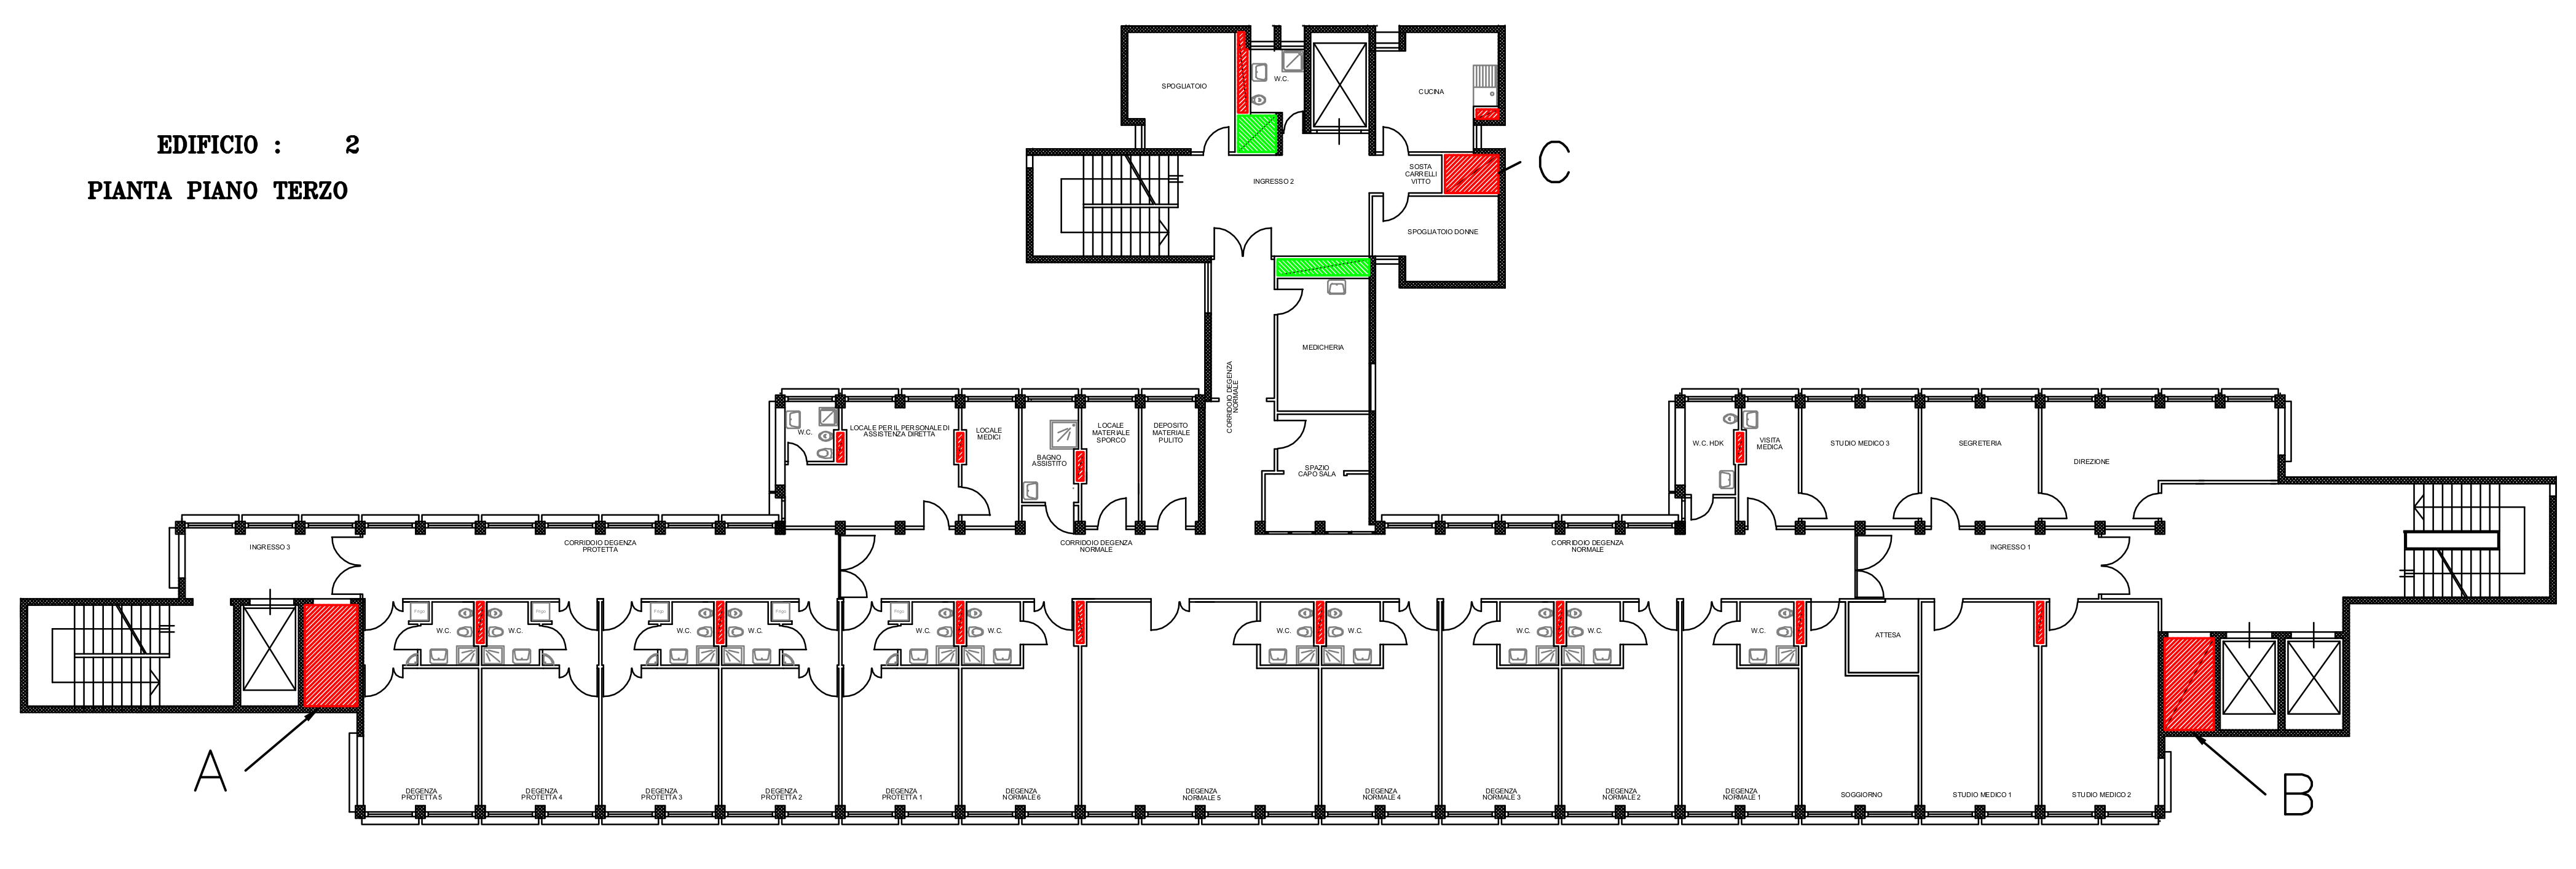
\includegraphics[width=\hsize]{6_4_cap/img/cavedi}
	\caption{Cavedi del Piano Terzo -- Corpo A}
	\label{img:cav}
\end{sidewaysfigure}
%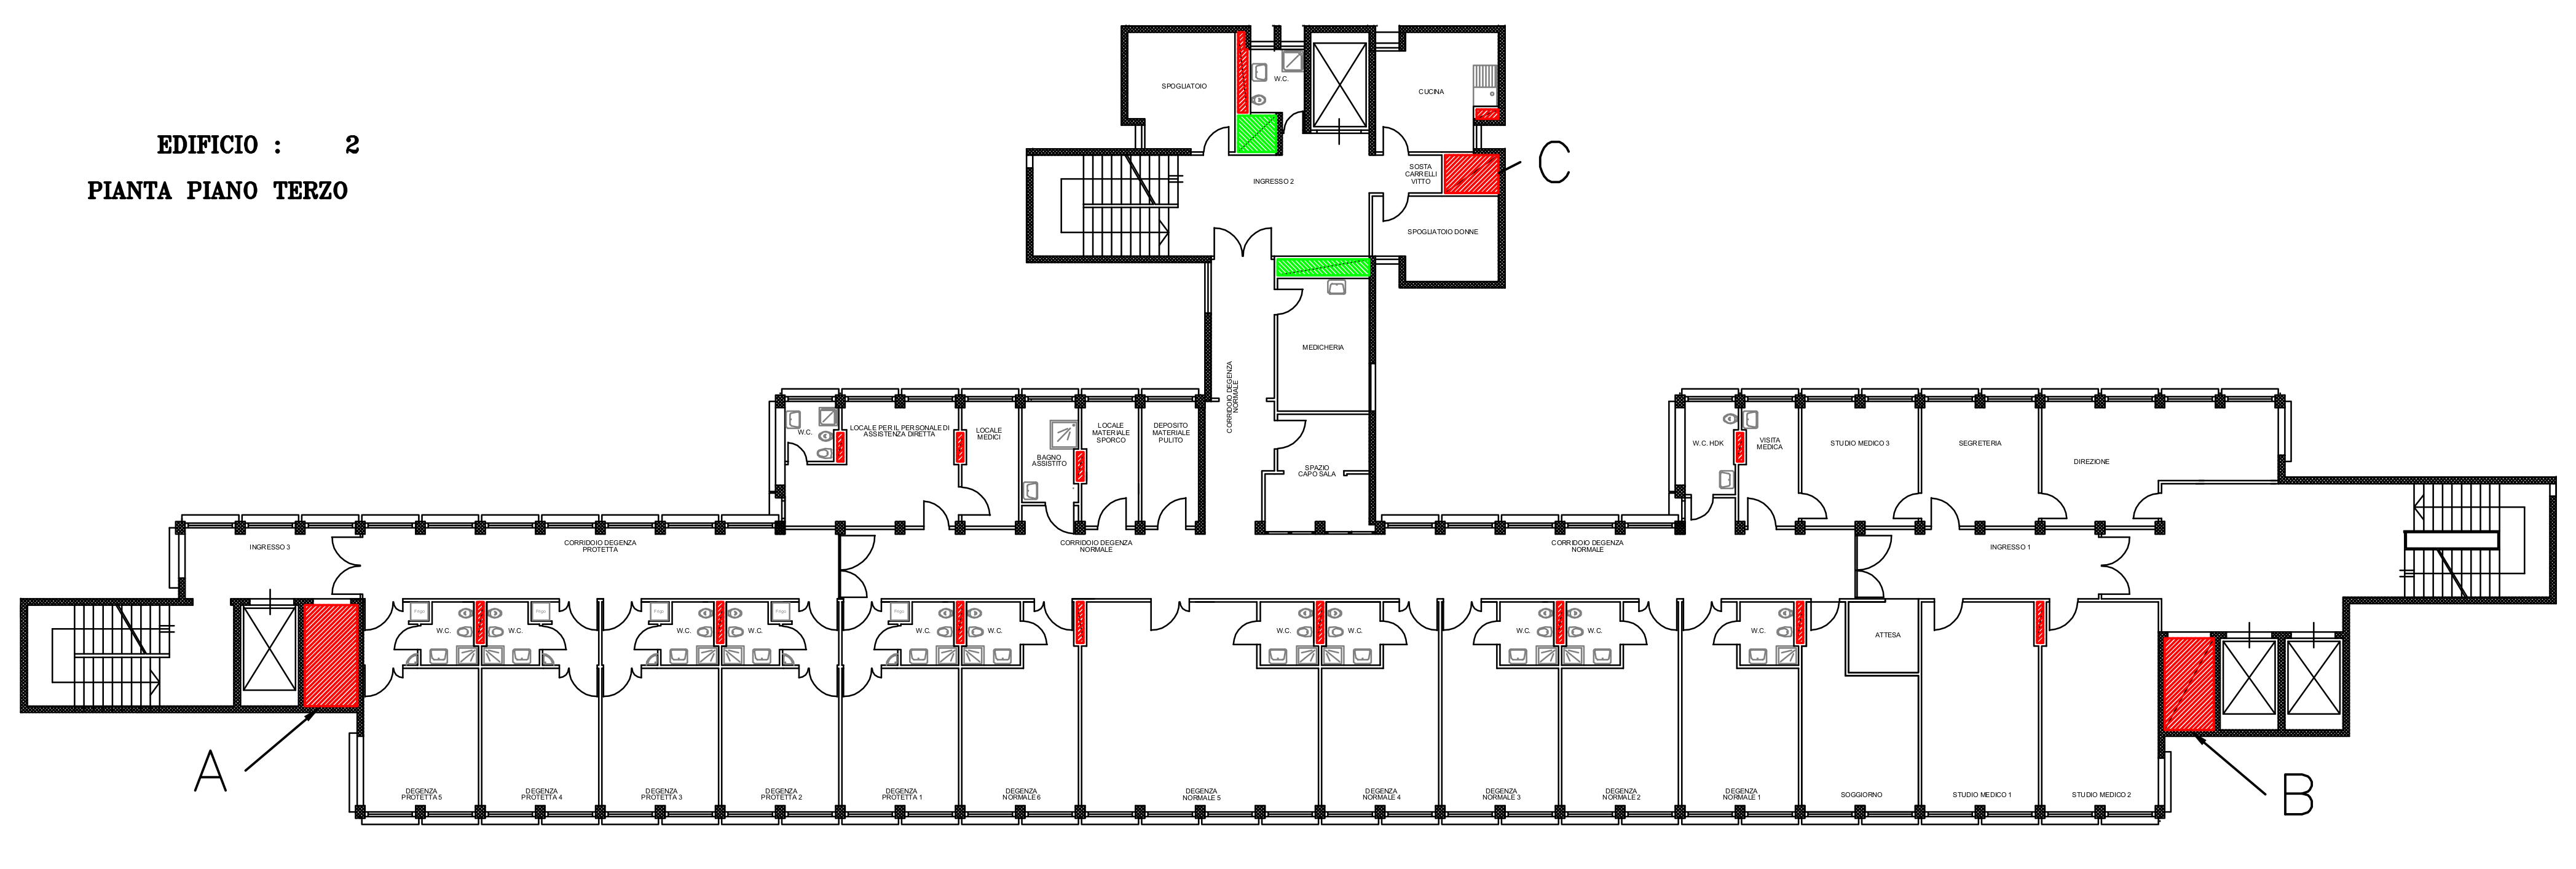
\includepdf{6_4_cap/img/cavedi}
I cavedi campiti in verde sono destinati alla rete elettrica. Tutti gli altri (in rosso) sono utilizzati dall'impianto idronico e aeraulico. In particolare, i 3 cavedi più grandi (i due adiacenti agli ascensori) e quello a destra nel torrino verranno utilizzati per le montanti dell'impianto a due tubi dei fancoil e dei radiatori. 

L'impianto dei fancoil è costituito da due tubi (una mandata e un ritorno). Vi saranno due montanti con una rete di distribuzione per ogni piano. Vista la configurazione essenzialmente longitudinale dell'edificio si è preferito costruire un circuito a \emph{ritorno inverso} con la montante di mandata che sale dal cavedio \textbf{A} e ritorna in quello \textbf{B}: in questo modo il \emph{ritorno inverso} è naturale. Per il torrino si è, invece, utilizzato il cavedio \textbf{C}. Lo \emph{switch} estate-inverno avviene in sottocentrale: in questo modo aumenta l'affidabilità di tutto l'impianto perché più semplice e con meno organi di regolazione.

L'impianto dei radiatori è pure a ritorno inverso e sfrutta i due cavedi \textbf{A} e \textbf{B}. 

I fancoil sono costituiti da una batteria alettata che scambia con l'aria in convezione forzata per la presenza di un ventilatore. Anche se vengono dimensionati per bilanciare il solo carico sensibile, quindi non si deve teoricamente formare la condensa, nella pratica lo fanno e pertanto possiedono sempre una vaschetta per l'eventuale acqua condensata. 

Scambiando per sola convezione, le temperature utilizzate nel caso estivo sono i famosi \num{7} - \n{12}{\degreeCelsius} e \num{50} - \n{45}{\degreeCelsius} nel funzionamento a caldo. 

I fancoil sono stati posizionati in tutti i locali eccetto i servizi igienici, spogliatoi e depositi vari.

Il dimensionamento è stato effettuato sfruttando la seguente relazione
\begin{equation}
	P=\dot{m}c\mathit{\Delta} T
\end{equation}
dove $P$ è la potenza termica sensibile, $\dot{m}$ è la portata d'acqua in \si{kg/s}, $c$ è il calore specifico dell'acqua e vale \n{4.2}{kJ/kgK} e il $\Delta T$ (differenza tra la temperatura di mandata e ritorno) vale \n{5}{\degreeCelsius}.

Per ogni locale (ovvero fancoil) si è calcolata la sua portata d'acqua necessaria per il funzionamento estivo e invernale. Il valore maggiore tra le due viene utilizzato per la scelta del diametro della tubazione. Alla fine si sommano tutte le portate per dimensionare la sotto-centrale. 

Per i radiatori si è proceduto nello stesso modo ricordando però \linebreak che $\Delta T=\SI{10}{\degreeCelsius}$.

Per entrambi gli impianti non si è provveduto ad inserire alcun organo di regolazione in quanto, essendo a \emph{ritorno inverso}, esso risulta bilanciato per natura. 

La tipologia dei fancoil è \emph{a soffitto} nel corpo A dove possibile (solitamente nelle degenze), \emph{a terra} nei corridoi e nel corpo C. In \vref{idr} è possibile vedere due figure della rete idronica dei due corpi. Si tratta di \emph{screenshot} dell'applicativo del software BIM della software-house C.A.T.S che permette, come è già stato detto precedentemente, di disegnare la rete, definire i carichi e calcolare la portata necessaria in ogni tratto dimensionandolo secondo criteri ben precisi. I rettangoli viola rappresentano i fancoil, quelli in rosso, invece, i radiatori. Come si nota, nelle degenze i fancoil non sono \emph{a soffitto} in quanto non esiste questa tipologia nel software. I risultati comunque non cambiano.

\begin{figure}
	\centering
	\subfloat[][\emph{Facciata meridionale}]{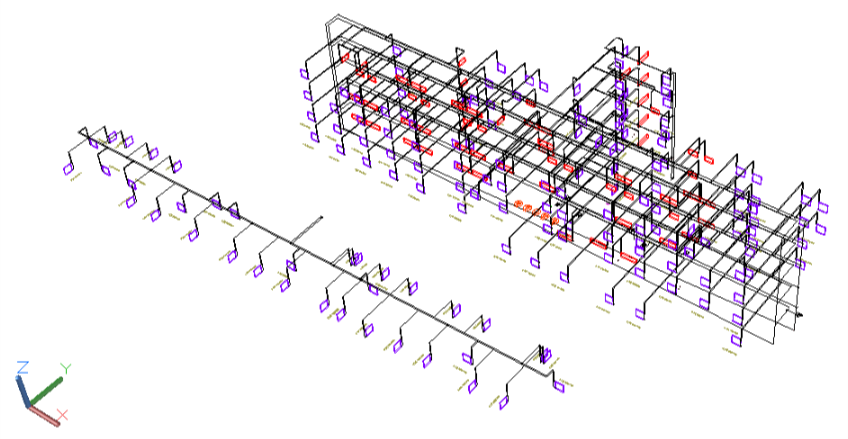
\includegraphics[width=\textwidth]{6_4_cap/img/idr1}\label{idr1}}\\
	\subfloat[][\emph{Facciata settentrionale}]{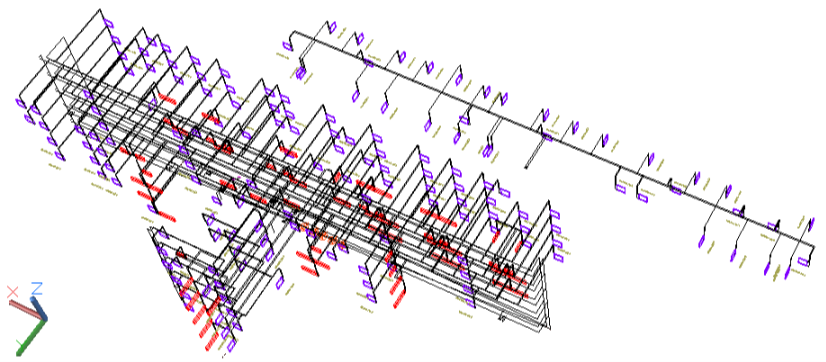
\includegraphics[width=\textwidth]{6_4_cap/img/idr2}\label{idr2}}
	\caption{Rete Idronica}\label{idr}
\end{figure}

\subsection{Impianto Aeraulico}
La portata di aria primaria per i corpi A e C è stata calcolata locale per locale utilizzando la \norvent. La rete aeraulica è stata disegnata su \textbf{CYPETHERM HVAC}. 

Non avendo spazio in cui posizionare le UTA, si sono usati dei recuperatori termodinamici. Tramite uno scambiatore a flussi incrociati, la portata di immissione e quella di estrazione vengono fatte entrare in contatto in modo tale che, in funzionamento estivo per esempio, la portata in uscita tenda a preraffreddare quella in ingresso. A valle di ciò, queste macchine possiedono anche un circuito a compressione di vapore le cui batterie alettate scambiano con la stessa portata di estrazione e immissione. Siccome le temperature dei due flussi sono vicine, queste pompe di calore hanno dei valori di efficienza (COP e EER) molto elevati.

Sono stati posizionati due recuperatori per piano nel corpo A (ma solo \num{1} al piano terra) nei pianerottoli delle scale antistanti i cavedi A e B. Nel corpo C vengono usati 4 recuperatori posizionati al piano \num{-1}.

Siccome queste reti aerauliche forniscono aria primaria ad un edificio ospedaliero, si vuole cercare di mantenere quanto è più pulito l'ambiente interno evitando infiltrazioni dall'esterno. Pertanto la portata di estrazione sarà minore di quella immessa in modo tale da generare un ambiente in sovrappressione rispetto l'esterno. Le velocità utilizzate per i canali di distribuzioni sono inferiori ai \n{3}{m/s} per contenere la rumorosità (oltre alle perdite di carico), mentre nei vari locali è stata diminuita a \n{2}{m/s}. Siccome l'impianto è \emph{misto}, la griglia di mandata dei fancoil viene sfruttata per immettere l'aria primaria della rete aeraulica in ambiente: in questo modo anche se la macchina idronica è spenta, l'impianto aeraulico può funzionare senza impedimenti o ostacoli. In \vref{aer} sono riportati due \emph{screenshot} di particolari della rete aeraulica dei due corpi mentre in \vref{img:aer} è presente la rete aeraulica intera del piano terzo come disegnata nell'applicativo \textbf{Load} di CYPE. 

\begin{figure}
	\centering
	\subfloat[][Vista meridionale]{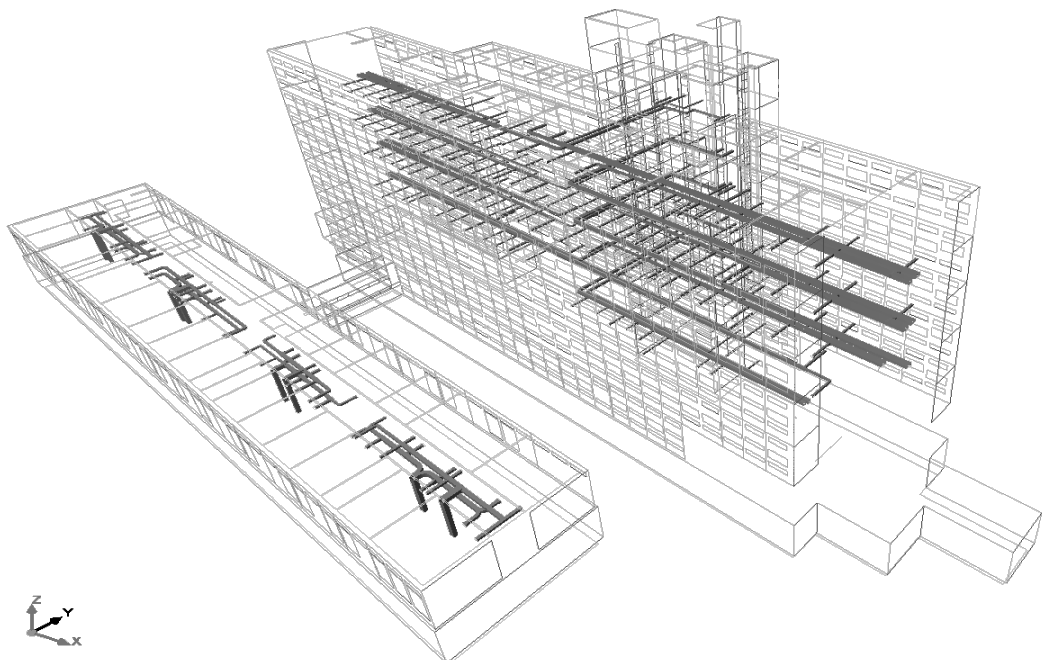
\includegraphics[width=0.9\textwidth]{6_4_cap/img/aer1}\label{aer1}}\\
	\subfloat[][Particolare del corpo C. Tramite il BIM è possibile disegnare e visualizzare in 3D.]{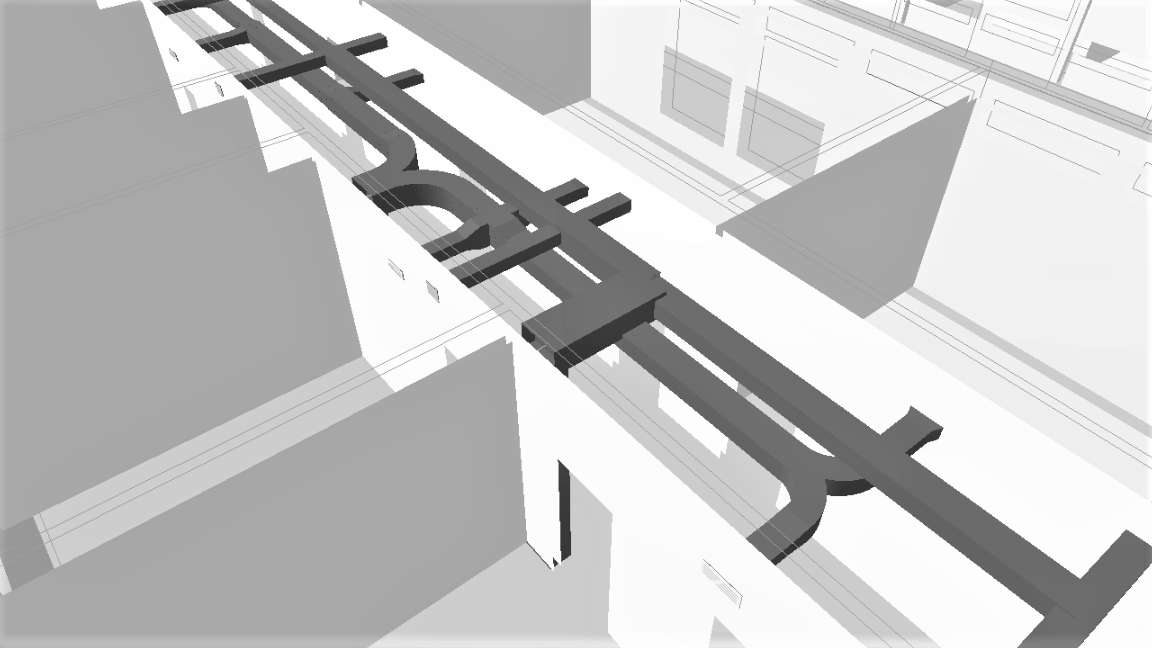
\includegraphics[width=0.9\textwidth]{6_4_cap/img/aer2}\label{aer2}}
	\caption[La rete aeraulica]{La rete aeraulica progettata con l'applicativo LOAD di CYPE}\label{aer}
\end{figure}
%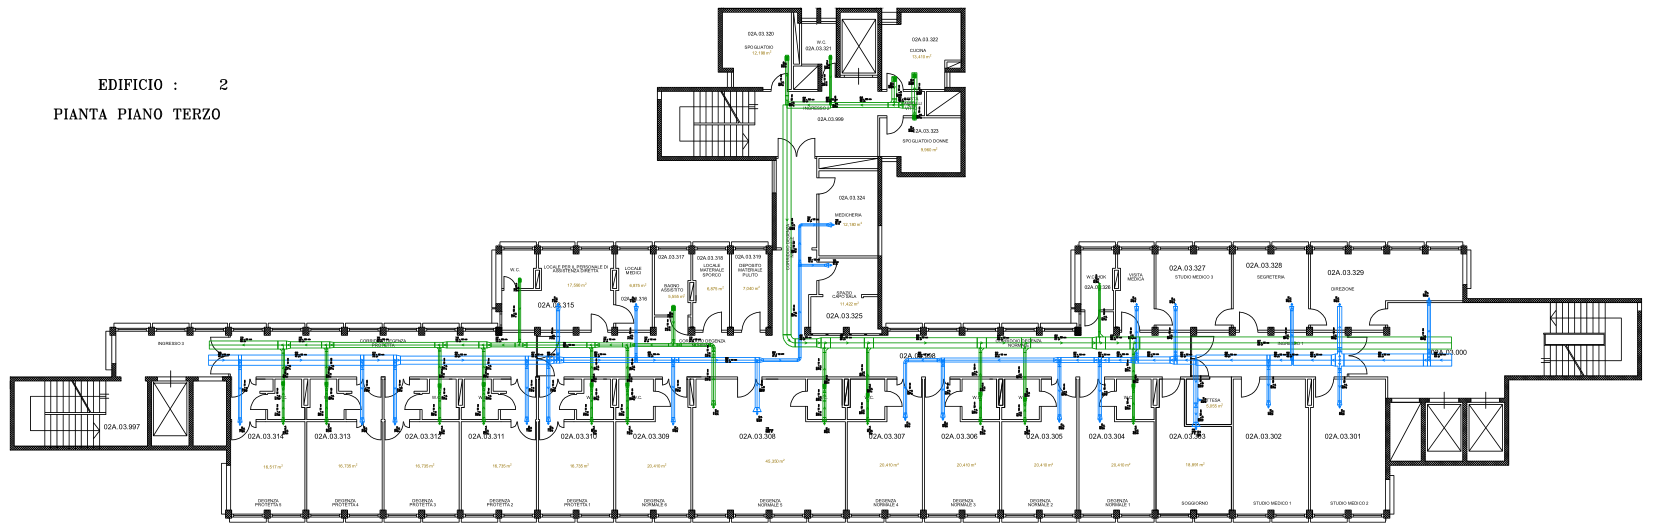
\includepdf{6_4_cap/img/aeraulica}
\begin{sidewaysfigure}
	\centering
	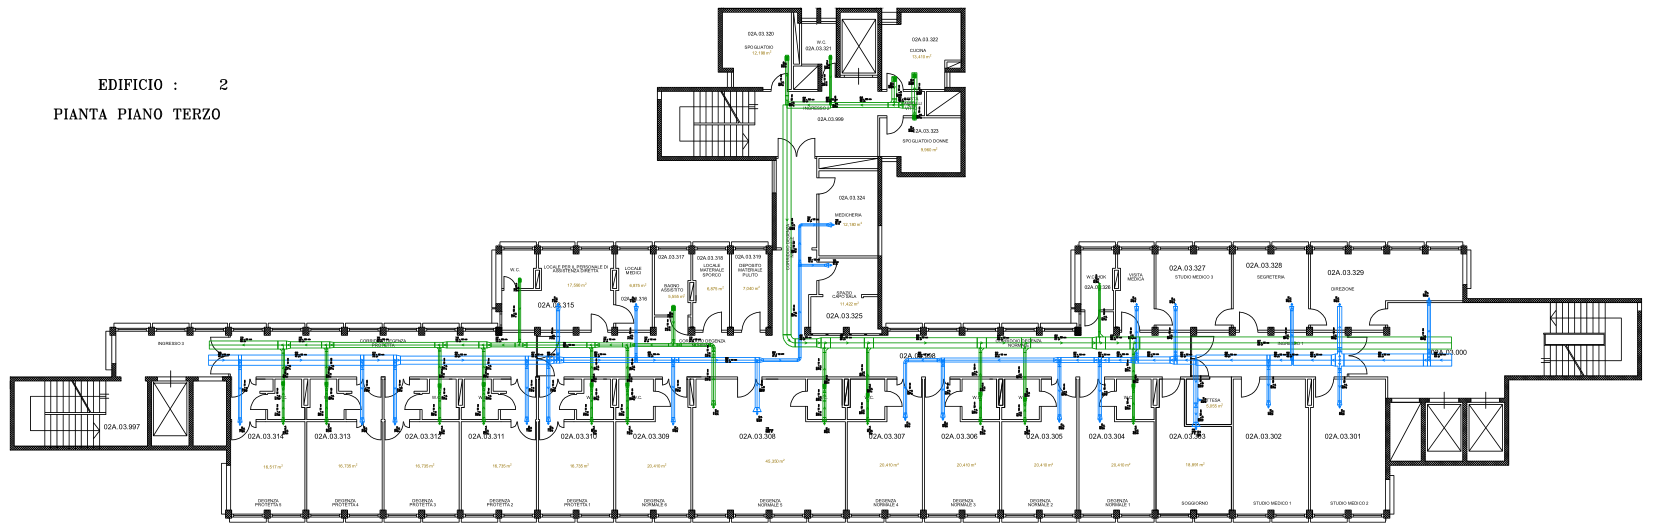
\includegraphics[width=\hsize]{6_4_cap/img/aeraulica}
	\caption{Rete Aeraulica Piano Terzo -- Corpo A}
	\label{img:aer}
\end{sidewaysfigure}
\clearpage
\section{L'impianto - Lato Sottocentrale}
Prima di procedere con la descrizione della sottocentrale che alimenta tutto il corpo di fabbrica dell'edificio 2, è doveroso elencare le utenze che usufruiranno dei servizi di acqua calda e refrigerata.
\begin{itemize}
	\item L'acqua calda è necessaria a diverse temperature per:
	\begin{itemize}
		\item Fancoil (\n{50}{\degreeCelsius});
		\item Radiatori (\n{80}{\degreeCelsius});
		\item Vecchi impianti, ovvero le UTA per il blocco operatorio, l'UTIC e l'emodinamica (\n{60}{\degreeCelsius});
		\item Acqua Calda Sanitaria (ACS).
	\end{itemize}
	\item L'acqua refrigerata è necessaria a \n{7}{\degreeCelsius} per:
	\begin{itemize}
		\item Fancoil;
		\item Vecchi impianti, ovvero le UTA per il blocco operatorio, l'UTIC e l'emodinamica.
	\end{itemize}
\end{itemize}
\subsection{Acqua Calda}
Come è già stato detto nel primo capitolo, in tutto il policlinico vi è una rete di presidio di acqua surriscaldata e refrigerata prodotta dai reflui termici del cogeneratore, caldaie e assorbitori. 

Per produrre acqua calda ad \n{80}{\degreeCelsius} si usa uno scambiatore dimensionato sulla $\dot{Q}_{\mathrm{risc,TOT}} = \sum \dot{Q}_{\mathrm{risc,i}}$ dove $\dot{Q}_{\mathrm{risc,i}}$ sono le potenze per il riscaldamento dei fancoil, UTA, radiatori delle varie zone termiche e dell'acqua calda sanitaria. La sommatoria non tiene conto delle potenze di ventilazione per i corpi A e C in quanto quel calore viene fornito (come anche nel caso estivo) dai recuperatori che possiedono un proprio impianto a compressione di vapore. Per questioni di sicurezza la $\dot{Q}_{\mathrm{risc,TOT}}$ viene aumentata di un \n{20}{\%} e vengono usati due scambiatori gemelli: in caso di guasto o manutenzione di una macchina, vi sarà l'altra ad assicurare la continuità del servizio.

In definitiva, essendo $\dot{Q}_{\mathrm{risc,TOT}}=\SI{600}{kW}$, sovradimensionando per sicurezza del \n{20}{\%} si ottengono \n{720}{kW}. 

Ogni scambiatore non verrà dimensionato sul massimo della potenzialità ma sui $2/3$ in quanto il picco si avrà solo in poche occasioni, per il resto del tempo (che rappresenta la maggior parte) ogni scambiatore lavorerà \emph{parzializzato}. Pertanto invece di dimensionare il singolo scambiatore sui \n{720}{kW}, si preferisce utilizzarne due da \n{480}{kW}. Nel funzionamento ordinario, sarà attivo un solo scambiatore mentre l'altro è di back-up. Nel caso ci siano esigenze particolari, si fa funzionare anche il secondo scambiatore. In caso di guasto o manutenzione (ordinaria e straordinaria) vi è l'altro scambiatore a garantire la continuità del servizio. Non bisogna dimenticare della presenza delle pompe di calore che comunque coprono una buona parte del carico. Quindi l'affidabilità e soprattutto la continuità del servizio sono garantite.

Il corretto funzionamento dello scambiatore (ovvero la produzione continua di acqua a \n{80}{\degreeCelsius}), viene assicurato da un termostato, posto nel ramo di mandata alle utenze, che, misurando continuamente la temperatura, invia un segnale ad una valvola a 3 vie a monte dello scambiatore (lato centrale) in modo tale da correggere la portata di acqua surriscaldata che fluisce nello scambiatore. 

In rispetto della \emph{Raccolta R} (elaborata dall'ISPESL -- Istituto Superiore per la Prevenzione e la Sicurezza del Lavoro -- e entrata in vigore nel \num{2011} con circolare INAIL -- Istituto Nazionale Assicurazioni e Infortuni sul Lavoro), a valle di entrambi gli scambiatori sono presenti tutti gli organi che assicurano \emph{Sicurezza}, \emph{Protezione} e \emph{Controllo} nei confronti di un impianto di generazione termica avente temperature di produzione massime non superiori a \n{110}{\degreeCelsius} e potenza nominale massima complessiva dei focolari superiore a \n{35}{kW}.

A monte e valle degli scambiatori sono presenti gli appositi strumenti per la contabilizzazione del calore:
\begin{itemize}
	\item flussometro: misura la portata di acqua che lo attraversa;
	\item 2 termostati: misurano la temperatura di mandata e ritorno e la comunicano ad un apposito controllore elettronico di temperatura (TC);
	\item TC: calcola la potenza utilizzata e la comunica al sistema informatico della sottocentrale. 
\end{itemize}
Solo con l'ausilio di questi strumenti è possibile conoscere effettivamente la potenza utilizzata e, di conseguenza, controllare se il comportamento dell'impianto è in linea con le ipotesi di progettazione.

La distribuzione dell'acqua a \n{80}{\degreeCelsius} viene affidata ad una coppia di pompe inverterate che portano il fluido all'unico collettore del secondario della sottocentrale dove ogni gruppo-pompe, uno per ogni servizio, alimenta la propria rete. 

La produzione di acqua a temperature inferiori per le batterie di pre e post riscaldamento delle UTA è affidata a valvole miscelatrici presenti sulla mandata: queste valvole miscelano la giusta portata di ritorno (ad una temperatura inferiore) e ad \n{80}{\degreeCelsius} in modo tale da ottenere la temperatura desiderata. Un termostato presente sulla mandata agisce direttamente sulla suddetta valvola a 3 vie.

Per il servizio fancoil (a \n{50}{\degreeCelsius}) si è optato per uno scambiatore, invece della valvola miscelatrice, per evitare che acqua a \n{80}{\degreeCelsius} entrasse durante la miscelazione nella rete stessa dei fancoil. In questo caso, però, bisogna ricordare che suddetta rete funziona con acqua calda in inverno e refrigerata in estate quando, però, bisogna garantire anche il servizio di acqua calda per le batterie di post-riscaldamento delle UTA.

Sul collettore del secondario a \n{80}{\degreeCelsius} vi è innestato anche il gruppo pompe per i bollitori dell'acqua calda sanitaria. Per il loro dimensionamento è stata utilizzata la UNI 9182. Si è proceduto in questo modo:
\begin{enumerate}
	\item Sono stati considerati 130 bagni in tutto il corpo A e C;
	\item la norma prevede per gli ospedali da \num{130} a \num{150} \si{l/persona} al giorno ($q_n$);
	\item la durata del periodo di punta dei consumi di acqua calda per gli ospedali vale 4 ore ($d$);
	\item si è determinato il massimo consumo orario contemporaneo di acqua calda a \n{40}{\degreeCelsius} usando la \vref{qm} dove $q_1=150$, $N=130$, $d=4$ e i tre fattori riduttivi per la contemporaneità sono unitari;
	\item Si è calcolato il volume del \emph{preparatore} (ovvero il bollitore) usando la \vref{preparatore};
	\item Si è calcolata la potenzialità termica da fornire al bollitore tramite l'acqua a \n{80}{\degreeCelsius} usando la \vref{serpentino}.
\end{enumerate}

\begin{equation}
q_M=\frac{q_1\times N_1}{d_1}\times f_1 \times f_2 \times f_3
\label{qm}
\end{equation}

\begin{equation}
	V_c=\frac{q_M \times d_p(T_m-T_f)}{d_p+P_r}\times \frac{P_r}{T_c-T_f}
	\label{preparatore}
\end{equation}

\begin{equation}
	W=\frac{q_M \times d_p (T_m-T_f)\times 1.163}{d_p+P_r}
	\label{serpentino}
\end{equation}

I risultati sono i seguenti:
\begin{itemize}
	\item $V_c = \SI{4400}{l}$ e quindi si useranno 2 bollitori da \n{5000}{l} per aumentare l'affidabilità del sistema;
	\item $W= \SI{120}{kW}$ e quindi la portata d'acqua a \n{80}{\degreeCelsius} sarà $\dot{m}_w\approx\SI{3}{kg/s}$ per bollitore.
\end{itemize}

\subsection{Acqua Refrigerata}
La produzione di acqua a \n{7}{\degreeCelsius} è affidata ad un mix di macchine ordinate in base alla priorità nel seguente elenco:
\begin{itemize}
	\item Assorbitori che sfruttano la rete di acqua surriscaldata di presidio;
	\item Pompe di calore con impianto geotermico.	
	\item Scambiatori che sfruttano la rete di acqua refrigerata di presidio;
\end{itemize}
Il cogeneratore ha \n{9}{MW} di reflui termici in estate di cui solo una parte vengono effettivamente utilizzati negli assorbitori i quali, al giorno d'oggi, non riescono a coprire il carico termico estivo di tutta la rete ospedaliera. Per questo motivo si è optata per l'installazione di un assorbitore in sottocentrale dedicato per il solo edificio 2: per sfruttare i reflui termici del cogeneratore che altrimenti verrebbero persi.

Le pompe di calore producono acqua refrigerata a \n{7}{\degreeCelsius} in estate e a \n{50}{\degreeCelsius} in inverno per i soli fancoil sul lato utenza, mentre scambiano con un apposito impianto geotermico.

Infine, gli scambiatori sfruttano la rete di presidio di acqua refrigerata per la fornitura del servizio in tutto l'edificio. In caso di guasto o manutenzione di una delle macchine di cui sopra, gli scambiatori permettono comunque di erogare al \n{100}{\%} il servizio.

Il mix così descritto permette di produrre acqua refrigerata con un'elevata affidabilità.
\subsubsection{L'assorbitore}
Di seguito è descritto il principio di funzionamento dei gruppi ad assorbimento, evidenziandone gli aspetti più significativi sotto il profilo impiantistico ed energetico. 

Le \emph{AHP} -- Absorption Heat Pump -- sebbene già sviluppate in età pioneristica (a partire dal 1860 circa), dopo un certo successo iniziale di mercato, con l'avvento dell'energia elettrica, furono soppiantate dalle \emph{EHP} -- Electric Heat Pump. Rispetto a queste ultime, le AHP presentano considerevoli vantaggi di tipo energetico ed ambientale, cui possono in alcuni casi accompagnarsi interessanti risparmi sui costi di esercizio.

Il principio di funzionamento si basa sulla capacità di particolari soluzioni chimiche (ottenute mescolando una sostanza \emph{refrigerante} ed una \emph{assorbente}) di assorbire continuativamente il vapore di refrigerante proveniente dall'evaporatore di una macchina frigorifera permettendo dunque che in quest'ultima l'evaporazione, e quindi l'effetto frigorigeno desiderato, siano continui.

Sono ancora presenti l'evaporatore ed il condensatore ma la compressione del vapore non è meccanica (scompare il compressore) ma termochimica (è presente un assorbitore/generatore). Al pari delle EHP, le AHP utilizzano l'evaporazione di un fluido \emph{refrigerante} per sottrarre energia termica dall'ambiente da climatizzare. Il refrigerante vaporizzato viene assorbito da una soluzione acquosa in cui è presente l'assorbente. Le coppie di fluidi di lavoro (refrigerante/assorbente) attualmente più utilizzate sono ammoniaca/acqua e acqua/bromuro di litio che è la più diffusa nelle macchine attualmente in commercio. Accanto alle funzioni di evaporazione ed assorbimento, per assicurare il funzionamento ciclico della macchina occorre far sì che l'assorbente, diluito nel refrigerante, riacquisti la sua capacità assorbente iniziale. A questo scopo viene introdotta una fase di rigenerazione: dall'assorbitore la miscela ricca di refrigerante viene inviata in un ulteriore dispositivo, il generatore, dove, per effetto di un'adduzione d'energia termica, si impoverisce di refrigerante; in tal modo, si ripristinano le condizioni iniziali delle fasi di evaporazione ed assorbimento.

Nelle applicazioni attuali si distinguono due tipologie di macchine ad assorbimento: quelle ad \emph{alimentazione indiretta} e quelle a \emph{fiamma diretta}.

Alla prima categoria appartengono quelle macchine che utilizzano come fluido caldo di alimentazione acqua surriscaldata (\num{115} + \n{132}{\degreeCelsius}, o anche temperature molto inferiori) o vapor d'acqua (\num{60} + \n{80}{kPa}) che fluisce all'interno di uno scambiatore posto nel generatore. La produzione del fluido caldo può essere affidata ad un generatore di vapore, oppure è possibile utilizzare i reflui termici di motori endotermici o dei processi industriali.

Nei gruppi a fiamma diretta, nel generatore avviene il riscaldamento direttamente con un bruciatore, solitamente alimentato a gas naturale.

Le prestazioni delle AHP decrescono al crescere della temperatura media cui è ceduta la potenza termica dell'assorbitore e del condensatore. Ciò ha in generale imposto l'adozione della condensazione ad acqua anziché ad aria. Ovviamente la temperatura dell'acqua resa disponibile dalla torre condiziona fortemente la resa frigorifera delle AHP: quest'ultima si riduce del \n{20}{\%} per un incremento di temperatura dell'acqua di raffreddamento di soli \n{2}{\degreeCelsius}.

A causa dei più bassi COP realizzabili dalle AHP rispetto alle macchine a compressione di vapore condensate ad acqua (tipicamente \num{0.6} + \num{0.7} le prime, \num{3} + \num{5} le seconde), il fabbisogno d'acqua di raffreddamento è in generale notevolmente superiore (\num{1.5} + \num{2.1} volte) rispetto a quello di una corrispondente macchina a compressione di vapore. 

L'adozione delle torri di raffreddamento evaporativo da un lato permette di avere l'acqua di raffreddamento del condensatore e dell'assorbitore in un livello di temperatura abbastanza basso, \num{28} + \n{34}{\degreeCelsius}, da un altro rappresentano un ulteriore complicazione del sistema. Si ha, inoltre, l'introduzione di una fonte di rumore in una macchina che è di per sè molto silenziosa. Comunque, per macchine di taglia elevata, i costi di abbattimento del rumore per le AHP rimangono inferiori rispetto a quelli delle macchine a compressione di vapore. 

Nelle macchine a \emph{semplice effetto} o \emph{monostadio}, il COP, a causa delle irreversibilità presenti, è sempre inferiore a \num{1} con valori intorno a \num{0.7} per le macchine ad alimentazione indiretta (tipicamente ad acqua a \num{80} + \n{90}{\degreeCelsius} per le macchine a acqua e bromuro di litio e a vapore a \num{130} + \n{140}{\degreeCelsius} per quelle ad ammoniaca) ed intorno a \num{0.6} per quelle a fiamma diretta. La limitazione sul valore del COP è superata con macchine più complesse a \emph{doppio effetto} o \emph{bistadio}. In estrema sintesi, rispetto allo schema della macchina monostadio è inserito un secondo generatore a più alta temperatura e pressione (\emph{generatore ad alta temperatura}) che interagisce con l'esterno in modo diretto (fiamma diretta) od indiretto (alimentazione a vapore oltre \n{180}{\degreeCelsius}).

Il vapor d'acqua prodotto internamente a questo generatore ha una temperatura sufficientemente elevata per essere impiegato nel secondo stadio (\emph{secondo generatore}); in esso, a temperatura e pressione prossime a quella del monostadio, condensando realizza, senza ulteriore spesa, un'ulteriore concentrazione/generazione. Da questo punto in poi il circuito è equivalente a quello del monostadio con la differenza che nell'AHP a doppio stadio un'unità di massa prodotta nel generatore ad alta temperatura può fare evaporare , rispetto al monostadio, un'ulteriore unità di massa di refrigerante nel generatore a bassa temperatura, e quindi avere nell'evaporatore l'evaporazione di due unità di massa di refrigerante. il COP massimo raggiunto da queste apparecchiature si aggira intorno a \num{1.3} per le macchine ad alimentazione indiretta e intorno all'unità per quelle a fiamma diretta.

In definitiva, si può affermare che, rispetto alle tradizionali apparecchiature a compressione di vapore, gli assorbitori offrono i seguenti vantaggi:
\begin{itemize}
	\item rispetto delle normative ecologiche per il mancato impiego di fluidi clorofluoroderivati;
	\item l'utilizzo dell'energia elettrica è per il solo azionamento degli organi ausiliari: ciò comporta una drastica riduzione, rispetto ai tradizionali gruppi elettrici:
	\begin{itemize}
		\item del fabbisogno di energia elettrica (nel rapporto \num{1} a \num{10});
		\item della potenza elettrica assorbita.
	\end{itemize}
	\item sostanziale assenza di parti in movimento, con drastica riduzione di vibrazioni e rumorosità, mentre i gruppi a compressione impongono spesso costose opere di insonorizzazione;
	\item buona durata ed affidabilità;
	\item ottime prestazioni ai carichi parziali.
\end{itemize}
Di contro ci sono alcuni svantaggi:
\begin{itemize}
	\item modesto COP;
	\item necessità di ricorrere ad acqua di torre per la condensazione, soprattutto per gli assorbitori ad acqua/bromuro di litio;
	\item per gli assorbitori ad acqua/bromuro di litio, la necessità di ricorrere ad un'accurata gestione e manutenzione per quanto riguarda la tenuta al vuoto, indispensabile per il loro corretto funzionamento e per evitare l'insorgenza di corrosione;
	\item accurato controllo della temperatura dell'acqua di raffreddamento del condensatore/evaporatore in quanto, nel caso in cui sia troppo bassa, rischia di solidificare il bromuro di litio (in relazione alla sua concentrazione). Infatti, sul ritorno dell'acqua di torre vi è termostato che misura la temperatura: nel caso in cui questa sia troppo bassa, agisce su una valvola miscelatrice posta sul ritorno dell'acqua di torre bypassando di fatto la torre di condensazione stessa e facendo tornare all'assorbitore/condensatore acqua calda.
\end{itemize}
Tornando nell'ambito progettuale di questo elaborato di laurea, avendo in estate i reflui termici del cogeneratore utilizzabili mediante l'acqua surriscaldata a \n{130}{\degreeCelsius}, si è preferito utilizzare un assorbitore.

Le caratteristiche della macchina, per quello che è stato detto nella teoria, saranno le seguenti: \emph{alimentazione indiretta}, \emph{bistadio} e come fluido \emph{acqua e bromuro di litio}. Si è fissato il COP ad un cautelativo \num{1.25}. 

L'assorbitore è stato dimensionato sul carico massimo estivo. Si spera che in questo modo sia possibile utilizzare quanti più reflui termici essendo questi gratuiti (in quanto il \emph{goal} del cogeneratore è la produzione di energia elettrica per il policlinico).

La potenza termica di raffreddamento è $\dot{Q}_{\mathrm{raff}}=\SI{730}{kW}$ e sovradimensionando di un coefficiente di sicurezza pari al \n{20}{\%} si ottiene $\dot{Q}_{\mathrm{raff}}=\SI{900}{kW}$ che sarà la potenzialità dell'assorbitore.

Scrivendo la relazione del COP,
\begin{equation}
	COP=\frac{\dot{Q}_{EV}}{\dot{Q}_{GE}}
\end{equation}
è possibile quantificare la potenza necessaria al generatore e quindi valutare la portata di acqua surriscaldata necessaria. 
\begin{align}
	\dot{Q}_{GE} &= \SI{720}{kW}\\
	\dot{m}_w &= \frac{\dot{Q}_{GE}}{c\ \mathit{\Delta} T}\label{Portata}\\
	\dot{m}_w&=\SI{5.7}{kg/s}\label{Portata:acquacalda}
\end{align}
nella \vref{Portata} si è fissato $\mathit{\Delta} T=\SI{30}{\degreeCelsius}$.

Siccome per gli assorbitori vale il seguente bilancio energetico
\begin{equation}
	\dot{Q}_{GE}+\dot{Q}_{EV}=\dot{Q}_{CO}+\dot{Q}_{ASS}
\end{equation}
sarà che la potenza da sottrarre al condensatore e all'assorbitore (e quindi da smaltire in atmosfera mediante la torre evaporativa) vale
\begin{equation}
	\dot{Q}_{CO}+\dot{Q}_{ASS}=\SI{1620}{kW}
\end{equation}
e quindi, per il solito coefficiente di sicurezza, si dimensionerà la torre evaporativa su una potenzialità pari a $\dot{Q}_{TORRE}=\SI{1900}{kW}$, il che necessita di una portata d'acqua pari a (con $\Delta T=\SI{5}{\degreeCelsius}$)
\begin{equation}
	\dot{m}_w\approx \SI{90}{kg/s}
\end{equation}

\subsubsection{La pompa di calore e l'impianto geotermico}
Il principio di funzionamento di tali sistemi si basa sul cambiamento di fase del liquido frigorigeno lungo il ciclo termodinamico che quest'ultimo compie. Il raffreddamento è in generale ottenuto dall'evaporazione del refrigerante ad una temperatura e ad una pressione che sono le più basse al'interno del ciclo. Queste ultime sono successivamente innalzate attraverso la compressione meccanica del fluido frigorigeno che alla fine di tale processo è vapore surriscaldato ad una temperatura e ad una pressione che sono le più alte all'interno del ciclo. Il riscaldamento, cioè la somministrazione d'energia termica dal sistema all'ambiente, è ottenuto attraverso il desurriscaldamento del fluido frigorigeno e la sua successiva condensazione. Il ciclo si completa attraverso l'espansione del suddetto fluido attraverso un apposito organo fino alle condizioni in cui ricomincia il processo d'evaporazione. Sono per quanto detto presenti quattro trasformazioni compiute attraverso quattro distinti componenti.

Dal medesimo ciclo termodinamico possono dunque ottenersi sia un impianto \emph{frigorifero} che un impianto a \emph{pompa di calore}. In entrambi i casi è possibile definire un COP (\emph{Coefficient Of Performance}). 

Per quanto riguarda il fluido refrigerante evolvente nell'impianto, è necessario che quest'ultimo abbia delle particolari caratteristiche termodinamiche, economiche e d'impatto ambientale, tra cui:
\begin{itemize}
	\item la possibilità che il ciclo termodinamico possa essere collocato nella regione dei vapori saturi. Ciò deve verificarsi anche a temperature molto basse senza che compaia la fase solida;
	\item una curva della tensione di vapore tale che non si generino eccessiva pressioni e depressioni rispettivamente al condensatore ed all'evaporatore;
	\item una variazione di entalpia d'evaporazione sufficientemente alta tale che, a parità di potenza termica scambiata, siano necessarie portate di refrigerante e quindi costi di compressioni contenuti;
	\item un volume specifico non troppo grande in modo tale che il lavoro di compressione, le dimensioni dei condotti e del compressore non eccedano;
	\item un costo d'acquisto ridotto, una bassa tossicità e una buona stabilità chimica rispetto ai materiali che costituiscono l'impianto;
	\item un basso impatto ambientale nei riguardi del \emph{buco dell'ozono} e dell'\emph{effetto serra}.
\end{itemize}
Riguardo a quest'ultimo punto, i fluidi frigorigeni moderni di più largo impiego sono dal punto di vista chimico degli HFC (\emph{Hydro Fluoro Carburi}: R407C, R410a, R134a, ecc\dots) composti in cui, per limitare il problema legato alla comparsa dell'ozono sui poli terrestri, è assente rispetto ai vecchi refrigeranti (CFC, HCFC) la molecola del cloro (ritenuta appunto fra i responsabili del \emph{buco dell'ozono}). Ultimamente l'attenzione è posta anche nello scegliere fluidi refrigeranti che limitino l'assorbimento della radiazione infrarossa e cioè l'effetto serra. L'R134a è, ad esempio, uno di quelli che maggiormente causa tale fenomeno.

Vengono di seguito illustrate le caratteristiche di funzionamento delle pompe di calore a compressione di vapore in base alla sorgente o pozzo d'energia termica utilizzata.

\paragraph{L'aria}
È quella utilizzata più frequentemente. Lo scambiatore di calore esterno all'ambiente da climatizzare è in questo caso caratterizzato da un'estesa superficie di scambio termico. Ciò è dovuto alla modesta efficienza della trasmissione del calore causata dal basso coefficiente di scambio termico di un aeriforme qual è l'aria in convezione forzata. Per questa ragione lo scambiatore esterno è generalmente costituito da una batteria alettata. 

L'efficienza della pompa di calore dipende moltissimo dalla temperatura ambiente. Nel caso invernale, per esempio, quanto più è bassa la temperatura esterna, tanto più diminuisce il COP quando invece il carico di riscaldamento dell'edificio aumenta.

Nel caso le temperature esterne invernali scendono continuativamente sotto o sono prossime allo zero, vi è il problema della formazione di \emph{brina} sulla batteria alettata esterna che provoca la diminuzione di superficie di scambio termico effettivamente utile. Ciò provoca un abbassamento dell'efficienza dell'evaporatore (sempre in caso invernale) e la fuoriuscita dallo stesso di una miscela di vapore e liquido di refrigerante. La risposta della centralina di controllo è un nuovo abbassamento della pressione di saturazione all'evaporatore (e quindi della sua temperatura di saturazione) che provoca una formazione di brina ancora più spinto. È necessario, quindi, effettuare lo \emph{sbrinamento}: riscaldare in qualche modo la batteria dell'evaporatore. Questo comporta \emph{discomfort} per l'utenza interna o, nel migliore dei casi, una semplice interruzione del servizio di riscaldamento.

Quindi, siccome il funzionamento di una pompa di calore dipende moltissimo dalle caratteristiche termodinamiche ambientali, si cercano altre forme di SET in cui la variazione di temperatura sia quanto più contenuta possibile. Al sud Italia l'impiego delle pompe di calore durante tutta la stagione invernale è molto più favorevole che al centro o al nord dove tipicamente nei mesi di gennaio e febbraio si rischia la formazione di brina.

\paragraph{L'acqua}
L'acqua può essere una sorgente (o pozzo) d'energia termica ottimale. Nel caso venga adottata la configurazione con torre evaporativa è affidata a quest'ultima il compito di raffreddare l'acqua proveniente dal condensatore. La torre, attraverso la saturazione dell'aria di processo raffredda per effetto dell'evaporazione l'acqua proveniente dal condensatore. La saturazione è ottenuta grazie alla fine nebulizzazione dell'acqua di processo che può appartenere ad un circuito separato da quello del condensatore, oppure provenire direttamente da quest'ultimo. Ovviamente il potenziale di raffreddamento è limitato e rappresentato, nel caso ideale di efficienza unitaria della torre evaporativa, dalla temperatura di bulbo bagnato dell'aria di processo proveniente dall'esterno. Nella realtà l'efficienza delle torri evaporative è ben lontana dal \n{100}{\%}. Notevole attenzione va prestata alla manutenzione del sistema necessaria anche per scongiurare il pericolo dell'insorgenza di funghi e infezioni come la \emph{legionella} dovuti alla presenza del necessario ristagno d'acqua. L'aria è movimentata da un ventilatore che insieme al consumo d'acqua e alla suddetta manutenzione rappresentano i costi di esercizio della torre.

Nel caso in cui sia possibile utilizzare la configurazione con \emph{circuito aperto} i vantaggi sono molteplici. Innanzitutto l'inerzia termica della sorgente (mare, fiumi, laghi, falda, ecc\dots) garantisce in generale una temperatura stabile per gran parte dell'anno, le fluttuazione sono infatti estremamente lente, dell'ordine di qualche giorno per grado di variazione. Un ulteriore vantaggio è rappresentato, a seconda della stagione, dall'elevata o bassa temperatura della sorgente. In estate ad esempio nel caso dell'acqua di mare, basta scendere di circa \n{10}{m} sotto la superficie per trovare una temperatura compresa tra gli \num{8} e i \n{12}{\degreeCelsius}.

\paragraph{L'energia solare}
In inverno uno dei principali vantaggi nell'utilizzo della radiazione solare come sorgente d'energia termica nelle pompe di calore è l'elevato valore della temperatura rispetto alle altre sorgenti con conseguente aumento del COP. Rispetto all'utilizzo dell'energia solare senza pompa di calore, l'efficienza e la potenza termica unitaria dei collettori solari è incrementata dalla minor temperatura richiesta al collettore. Vista l'enorme variabilità della radiazione solare durante la giornata, è molto importante accoppiare un impianto di collettori solare ad un accumulo termico correttamente dimensionato.

\paragraph{Il terreno}
La temperatura del terreno ad una certa profondità si stabilizza ad un valore molto prossimo a quello della media annuale della temperatura dell'aria. Ad elevate profondità, invece, entra in gioco l'energia termica endogena. Infatti, oltre i \n{30}{m} di profondità si riscontra in media un incremento di temperatura di circa \n{1}{\degreeCelsius} ogni \n{30}{m}. La temperatura del terreno è quindi più stabile di quella dell'aria esterna, non risente delle oscillazioni giornaliere, le variazioni di temperatura sono smorzate e ritardate di fase. Il tutto è tanto più vero quanto maggiore è la profondità. Le pompe di calore che utilizzano il terreno come sorgente di calore in inverno e pozzo di calore in estate sono dunque vantaggiose.

Questo tipo di pompe di calore prevede l'interramento di tubi di adeguata lunghezza attraverso due differenti tecniche: tubi orizzontali o tubi verticali. I sistemi a tubi orizzontali vengono interrati a piccola profondità (\num{0.8} + \n{1.5}{m}) trovando posto di solito sotto un'ampia superficie sgombra da edifici. I tubi devono resistere alla corrosione per periodi molto lunghi. Per questo motivo in passato si sono utilizzati spesso tubi in rame, mentre più recentemente si preferisce ricorrere a materie plastiche come il \emph{polietilene ad alta densità} ed il \emph{polibutilene rinforzato}. Le materie plastiche mentre risolvono il problema della corrosione e diminuiscono i costi, sono ovviamente caratterizzate da minori conduttività termiche rispetto ai metalli.

I sistemi a tubi verticali, invece, utilizzano una o più perforazioni con profondità variabili da valori minimi di \n{10}{m} a valori massimi che possono superare i \n{200}{m}. A tali profondità le temperature del terreno non risentono quasi più degli effetti superficiali. Inoltre la superficie in pianta richiesta è molto ridotta rispetto al caso precedente. Si possono utilizzare le stesse profondità dei pali di fondazione dell'edificio oppore raggiungerne maggiori. 

Le macchine che adottano tale tecnologia possono utilizzare un fluido secondario all'interno del circuito di tubi immerso nel terreno, che può essere acqua nei climi più miti o una miscela acqua-fluido anticongelante in quelli più rigidi. I fluidi anticongelanti più utilizzati sono il metanolo, l'etanolo e il glicol propilenico. In alternativa le macchine possono essere ad espansione diretta se utilizzano viceversa direttamente il fluido refrigerante nel circuito immerso nel terreno.

\vspace{1em}
Nella progettazione della sottocentrale si è stati obbligati ad utilizzare come sorgente/pozzo di energia termica il terreno.

Innanzitutto è stato necessario capire come modellare il terreno. In assenza di dati, sono stati utilizzati quelli dell'adiacente ``Istituto Nazionale Tumori - IRCCS \emph{Fondazione G. Pascale}'' in cui è stato costruito un campo geotermico e per l'occasione sono stati effettuati dei carotaggi per la valutazione del sottosuolo.

I dati ricavati relativi al terreno sono:
\begin{itemize}
	\item conducibilità termica: $\lambda = \SI{0.79}{W/mK}$;
	\item temperatura indisturbata: $T_g=\SI{15.4}{\degreeCelsius}$
	\item capacità termica: $c=\SI{1.5}{MJ/m^3K}$
\end{itemize}

La difficoltà nella progettazione del campo geotermico risiede nella complessa valutazione di scambi energetici che il terreno ha con il resto dell'ambiente. Infatti, la temperatura del terreno dipende da 3 tipologie di fenomeni:
\begin{itemize}
	\item scambio d'energia con l'atmosfera: irraggiamento solare, eventi meteorici, trasmissione per convezione (a cui si aggiunge la variabilità del vento), calore estratto dalla vegetazione e calore scambiato con gli edifici soprastanti;
	\item scambio d'energia con gli acquiferi che, a seconda della stagione, possono apportare od estrarre energia;
	\item apporto energetico legato al flusso geotermico.
\end{itemize}
Purtroppo anche considerando e studiando questi fenomeni singolarmente, il bilancio globale non è determinabile banalmente tramite sovrapposizione degli effetti in quanto è necessario tenere conto della mutua influenza. Sono necessari modelli matematici complessi, da sviluppare caso per caso.

La procedura di calcolo utilizzata per il dimensionamento delle sonde geotermiche verticali è quello proposto dalla ASHRAE: tale metodo, infatti, si rifà a quello analitico basato sulla teoria della sorgente cilindrica sviluppato da \emph{Ingersoll} e \emph{Zobel} nel 1954 e ripreso da \emph{Kavanaugh} e \emph{Rafferty} nel 1997.

Il modello analitico ha dato risultati utili per una buona progettazione del campo geotermico i quali vengono riassunti di seguito.
\begin{itemize}
	\item in fase di esercizio dell'impianto geotermico, il funzionamento della pompa di calore, sopratutto in condizioni di massimo carico, può provocare un decremento eccessivo della temperatura del terreno intorno alla sonda e dunque anche del fluido termovettore: tale situazione genera pericoli di gelo e stress meccanici tra terreno e sonda, che potrebbero minare l'incolumità della sonda stessa;
	\item per operare un corretto dimensionamento della sonda, è necessario conoscere i carichi termici dell'edificio e il loro andamento temporale, in particolare il carico medio annuale standard, il carico mensile massimo e quello orario di punta, sia nel caso invernale che estivo;
	\item gli impianti geotermici costituiti da molteplici sonde devono garantire distante reciproche sufficienti tra le stesse, in modo da garantire che i campi termici rispettivi non si influenzino reciprocamente. 
\end{itemize}
La relazione utilizzata dall'ASHRAE tiene conto della variazione temporale dei flussi termici scambiati tra sonda e terreno e quindi del differente significato che assume la resistenza del terreno al variare del periodo dell'oscillazione del flusso termico. Dal punto di visto matematico, si tiene conto di questo fenomeno facendo riferimento a tre ``impulsi termici'' a gradino di durata differente, mediante una semplice sovrapposizione degli effetti di breve, di medio e di lungo termine. Per ciascun gradino si introduce la resistenza termica del terreno corrispondente all'intervallo di tempo considerato; gli effetti dei tre impulsi vengono sommati, tenendo conto dei carichi termici corrispettivi.

Le relazioni, una per il caso invernale e l'altra per quello estivo, sono:
\begin{align}
	L_c&= \frac{\Phi_a R_{ga}+(\Phi_{lc}-W_{c})(R_b+PLF_mR_{gm}+R_{gd}F_{sc})}{T_0-\frac{T_{fi}+T_{fo}}{2}-T_p}\\
	L_h&= \frac{\Phi_a R_{ga}+(\Phi_{lh}-W_{h})(R_b+PLF_mR_{gm}+R_{gd}F_{sc})}{T_0-\frac{T_{fi}+T_{fo}}{2}-T_p}
\end{align}
dove:
\begin{description}
	\item[$\mathbf{L_c} \-- \mathbf{L_h}$] sono le lunghezze di perforazione necessarie per soddisfare rispettivamente il carico estivo (\emph{cooling}) od invernale (\emph{heating}) (il valore maggiore tra i due definisce la profondità di installazione da adottare), in \si{m};
	\item[$\mathbf{\Phi_a}$] è il flusso termico medio scambiato con il sottosuolo in un anno, in \si{W};
	\item[$\mathbf{\Phi_{lc}} \-- \mathbf{\Phi_{lh}}$] sono i carichi termici di progetto rispettivamente in raffrescamento ($\Phi_{lc}<0$) e in riscaldamento ($\Phi_{lh}>0$) dell'edificio, in \si{W};
	\item[$\mathbf{W_c} \-- \mathbf{W_h}$] sono le potenze elettriche assorbite dal compressore della pompa di calore al carico termico estivo ed invernale di picco, in \si{W};
	\item[$\mathbf{R_{ga}}$] è la resistenza termica lineare equivalente del terreno per un impulso annuale, in \si{mK/W}. Serve a tenere conto dell'andamento della temperatura del terreno sul lungo periodo, sostanzialmente identificabile con la durata dell'impianto. Viene calcolata per un tempo pari a \num{10} anni (\num{3650} giorni);
	\item[$\mathbf{R_{gm}}$] è la resistenza termica lineare equivalente del terreno per un impulso mensile, in \si{mk/W}. Tiene conto delle fluttuazioni stagionali nel carico. Il tempo di riferimento è pari a \num{10} anni più \num{1} mese (\num{3680} giorni);
	\item[$\mathbf{R_{gd}}$] è la resistenza termica lineare equivalente del terreno per un impulso della durata di un giorno o frazione, in \si{mK/W}. Esprime le fluttuazioni di brevissimo periodo. Il tempo di riferimento è pari a \num{3680.25} giorni, ovvero \num{6} ore in più rispetto a quello per $R_{gm}$.;
	\item[$\mathbf{R_b}$] è la resistenza termica per unità di lunghezza della sonda, tra fluido e bordo sonda, in \si{mK/W};
	\item[$\mathbf{PLF_m}$] è il fattore di carico parziale per il mese di picco;
	\item[$\mathbf{F_{sc}}$] è il fattore di perdita legato al possibile cortocircuito termico in sonda tra tubo di mandata e ritorno;
	\item[$\mathbf{T_0}$] è la temperatura del terreno indisturbato, in \si{K};
	\item[$\mathbf{T_{fi}} \-- \mathbf{T_{fo}}$] sono le temperature di ingresso e uscita della pompa di calore (riferite al casto estive oppure invernale), in \si{K};
	\item[$\mathbf{T_p}$] è la temperatura di penalizzazione, dovuta all'interferenza reciproca tra sonde attraverso il terreno (positiva in inverno e negativa in estate), in \si{K}.
\end{description}
Inserendo opportunamente i dati e considerando come $\mathrm{COP}=\num{4.8}$ e $\mathrm{EER}=\num{4.5}$ di una generica pompa di calore, si ottengono i seguenti dati:
\begin{itemize}
	\item con lunghezze di perforazione da \n{250}{m} è necessario utilizzare \num{44} sonde in \emph{PEad} DN40;
	\item un impianto di questa estensione ha come potenze di progetto (ovvero verso l'utenza) in estate $\dot{Q}_{geo,c}=\SI{192}{kW}$ e in inverno $\dot{Q}_{geo,h}=\SI{170}{kW}$ ovvero si riesce a coprire il carico annuale sensibile del corpo A e C.
\end{itemize}
A questo punto è stato necessario collocare opportunamente le sonde intorno all'edificio 2 facendo attenzione alle fondazioni, ai cunicoli e alle varie reti (idrauliche e elettriche) presenti. Le distanze utilizzate sono:
\begin{itemize}
	\item \n{4}{m} dalle fondazioni degli altri edifici;
	\item \n{7}{m} tra una sonda e l'altra.
\end{itemize}
Il campo geotermico è stato suddiviso in più zone, ognuna facente capo ad un collettore. 

Si riporta in \vref{img:geot} il campo sonde. Le campiture grige rappresentano gli edifici; i tratteggi si riferiscono a zone in cui non bisogna scavare: in particolare quello rosso rappresenta il cunicolo sotterraneo. Ogni cerchio ha un raggio di \n{7}{m} e rappresenta la sfera di perturbazione della rispettiva sonda. Le tubazioni di ogni zona (rappresentate con le lettere) sono in rosso mentre le due distribuzioni dalla centrale sono in nero. Le zone verdi rappresentano le sistemazioni a verde.
%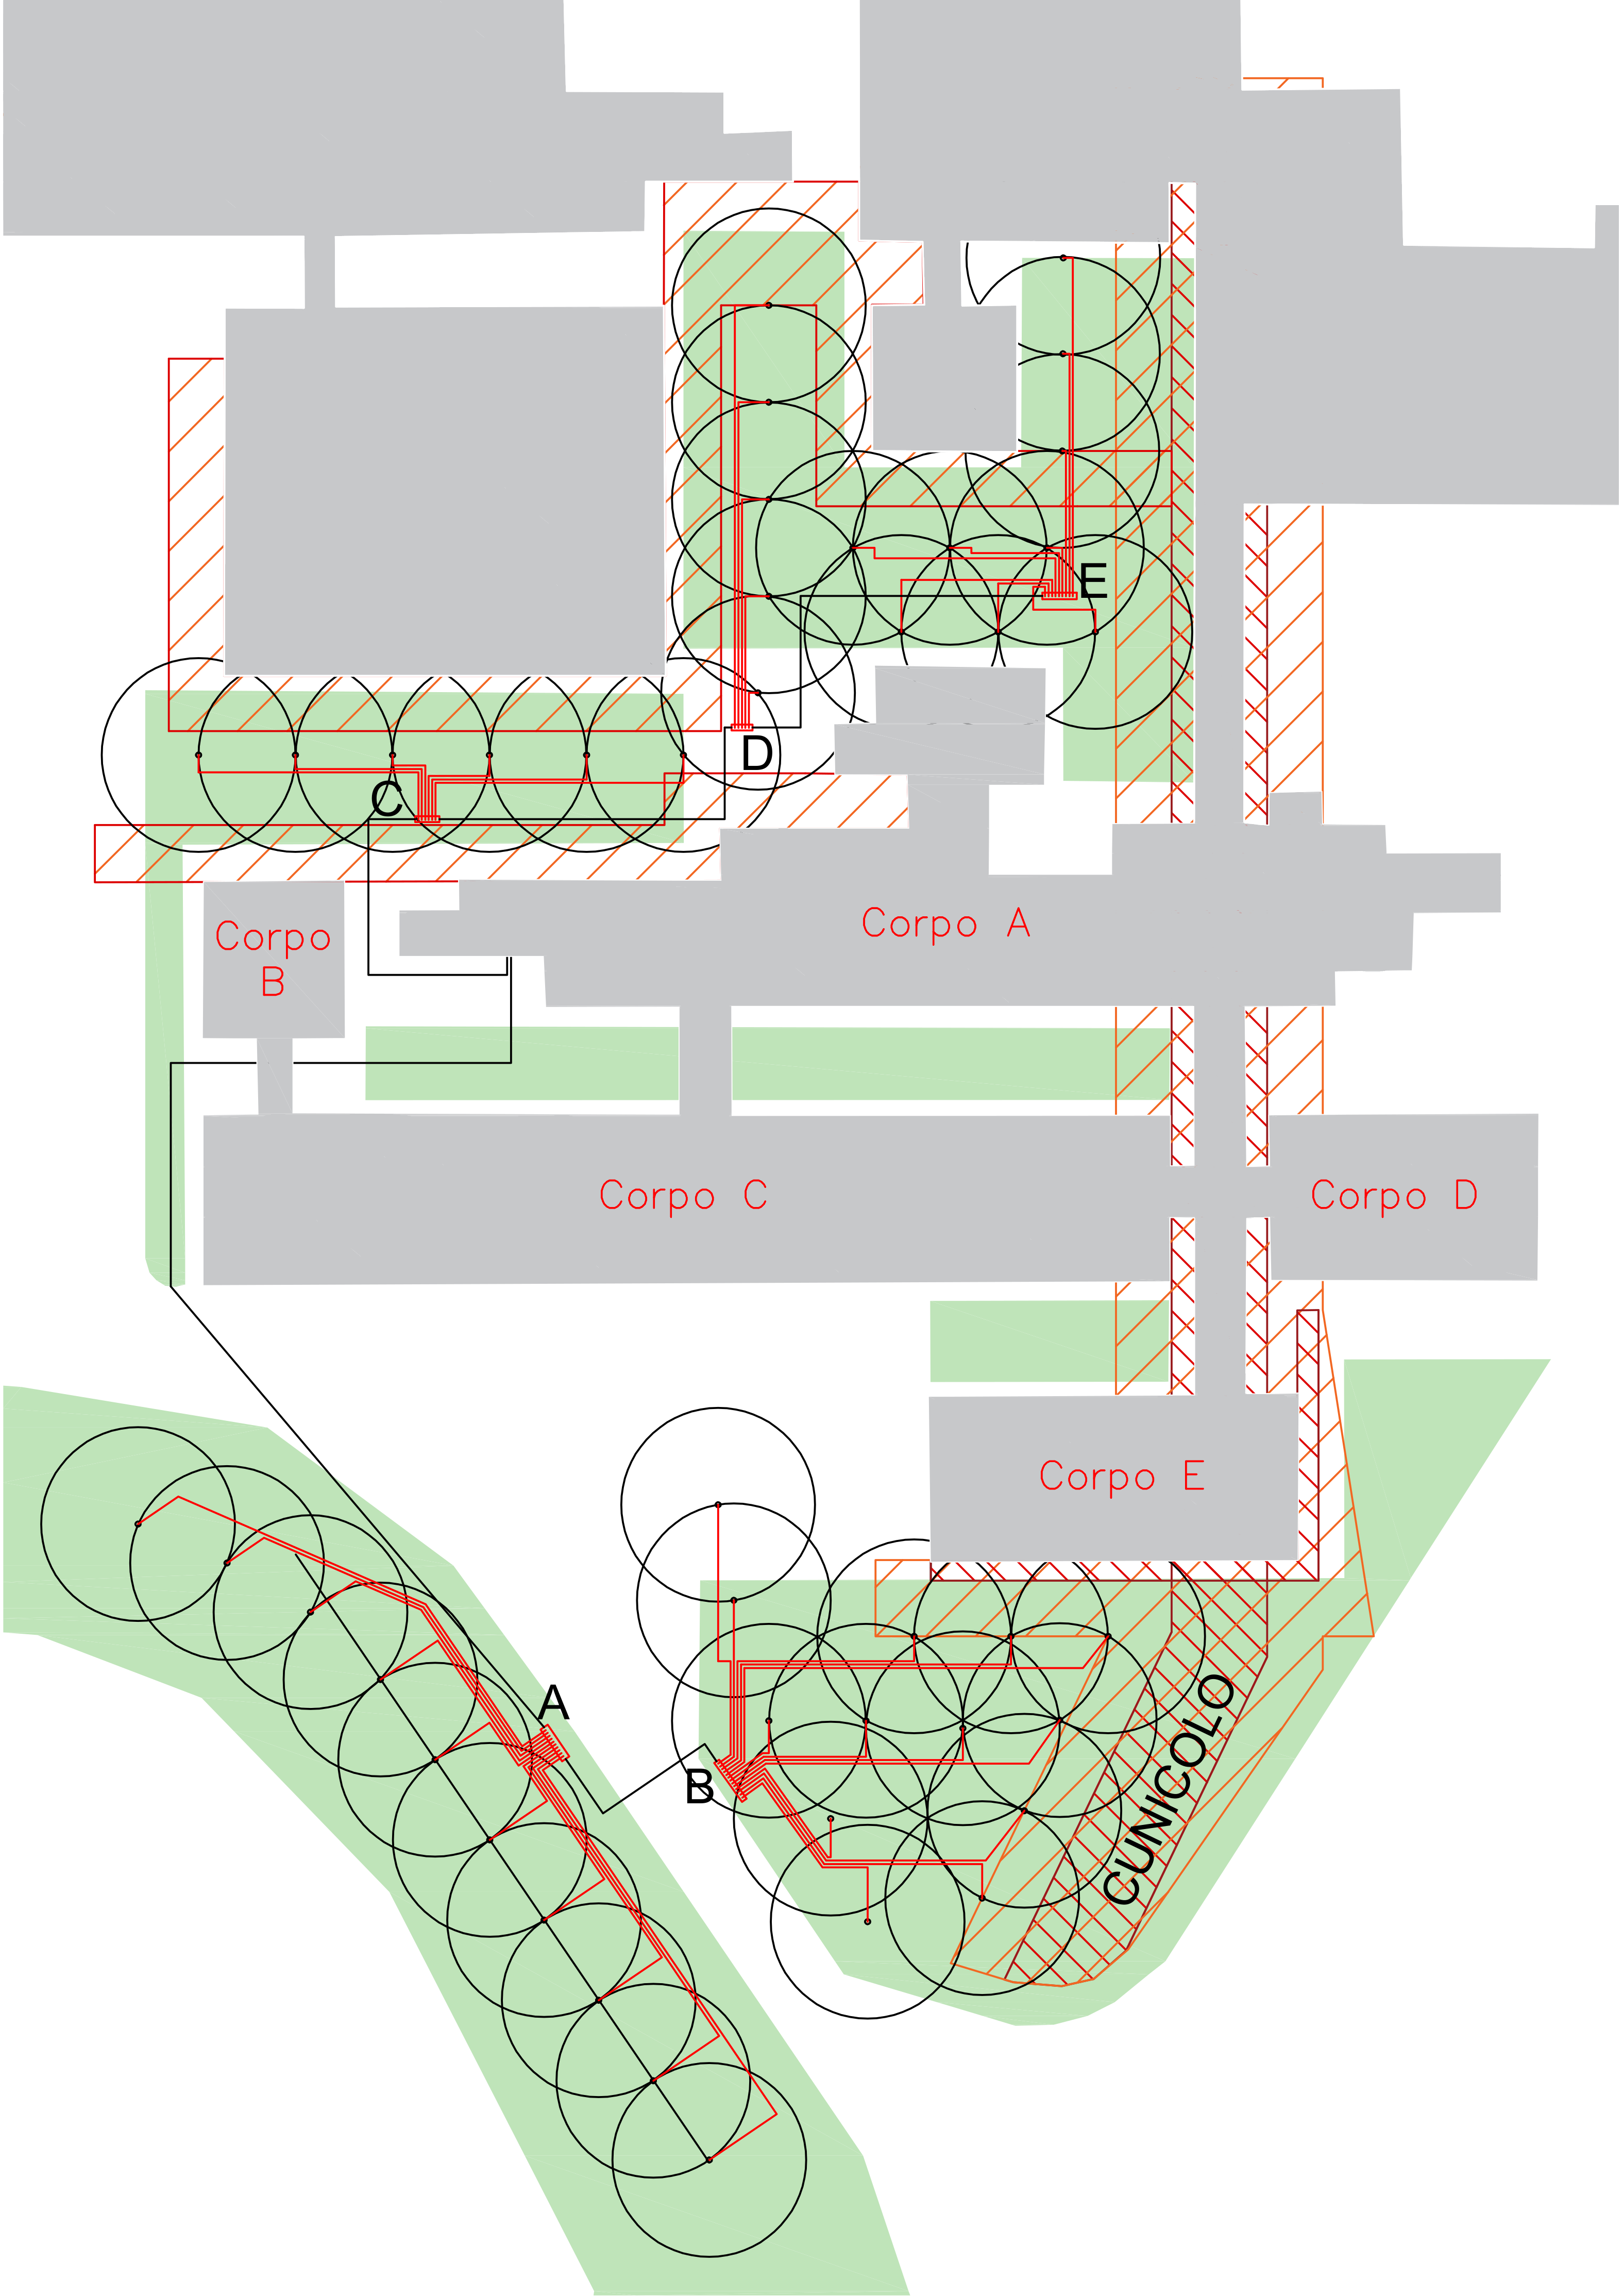
\includepdf{6_4_cap/img/geot}
\begin{figure}
	\centering
	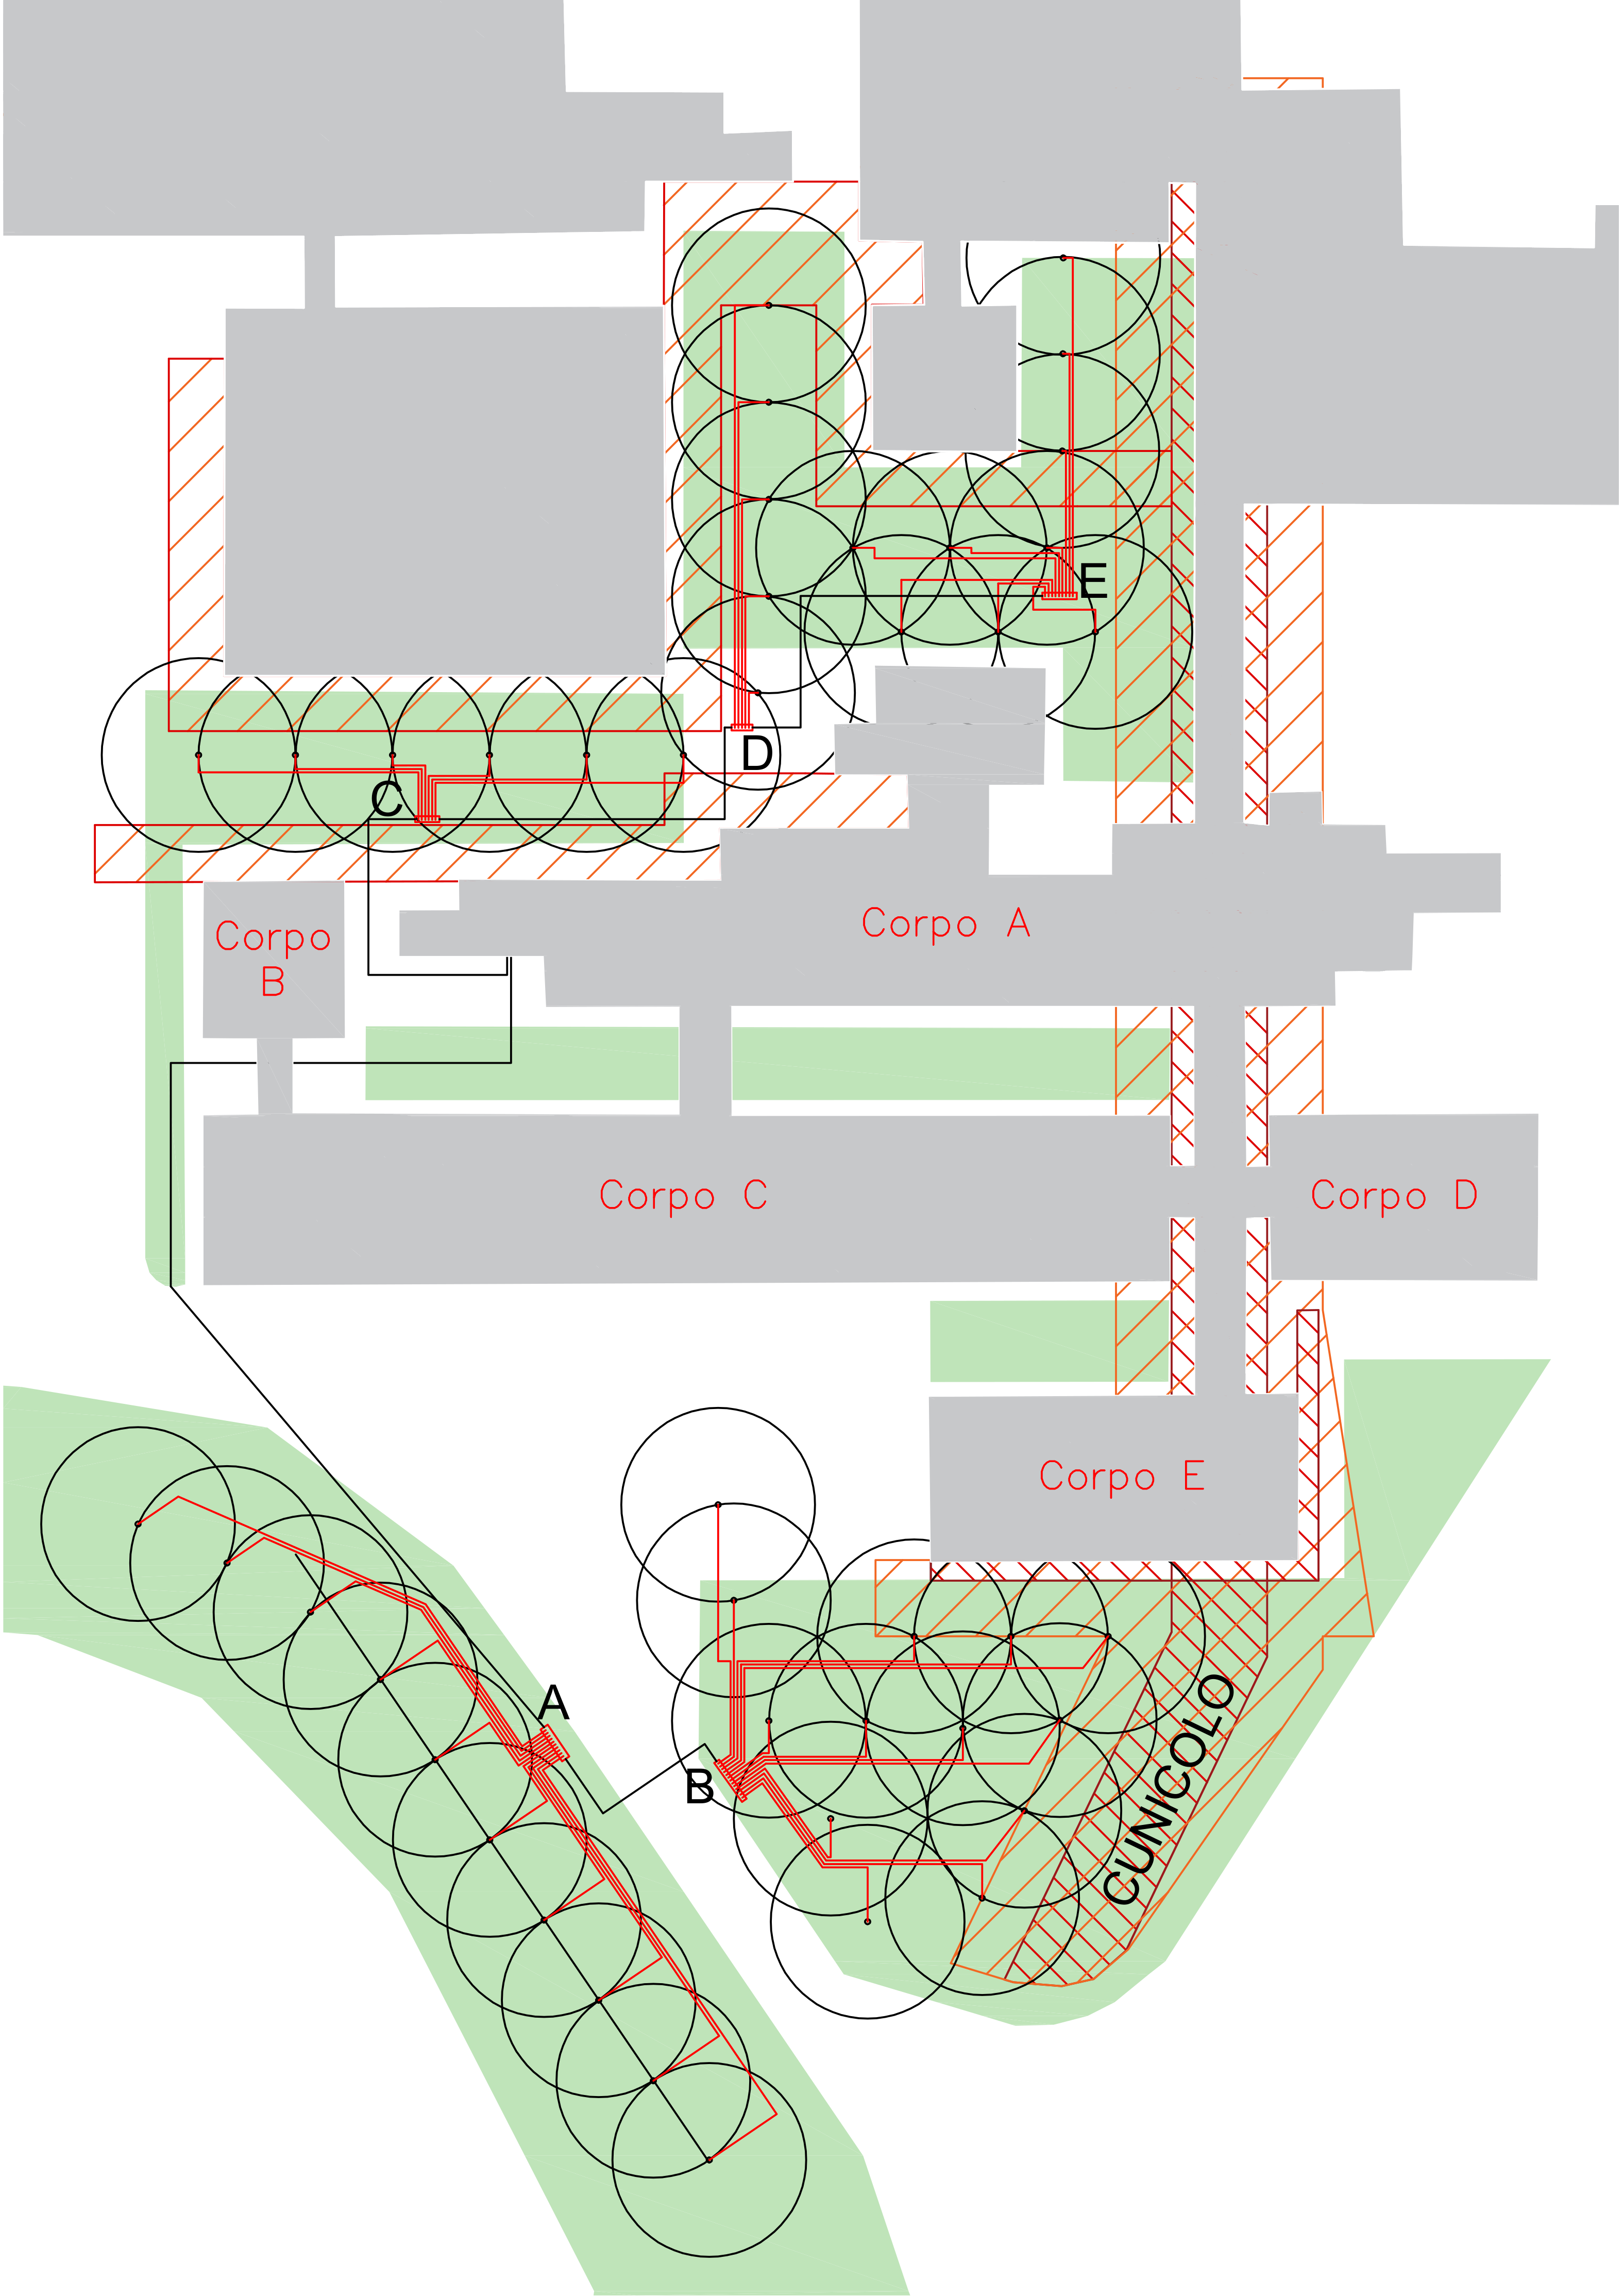
\includegraphics[width=\hsize]{6_4_cap/img/geot}
	\caption{Disposizione sonde geotermiche intorno all'edificio 2}
	\label{img:geot}
\end{figure}

Nella sottocentrale sono state utilizzate, quindi, due pompe di calore in parallelo capaci di rendere in inverno \n{90}{kW} e \n{100}{kW} in estate: questa scelta è stata effettuata in quanto in caso di carico massimo le due macchine riescono a sfruttare tutto il campo geotermico mentre in occasione dei carichi parziali, è possibile spegnerne una e lavorare sempre a pieno carico (e quindi col massimo dell'efficienza). Vista la numerosa dotazione di macchine per il freddo, avere due pompe di calore permette di aumentare l'affidabilità del sistema geotermico.
\subsubsection{Gli scambiatori}
Come nel caso dell'acqua calda, gli scambiatori raffreddano l'acqua sfruttando la rete di presidio di acqua refrigerata. Gli scambiatori rappresentano \emph{l'ultima spiaggia} in caso di malfunzionamenti del gruppo ad assorbimento e delle pompe di calore.

Essendo l'ultimo \emph{strumento} disponibile in sottocentrale per \emph{il freddo}, si è deciso di dimensionare la coppia di scambiatori sul massimo carico estivo tenendo conto del solito coefficiente di sicurezza del \n{20}{\%} e di futuri ampliamenti. Quindi essendo $\dot{Q}_{\mathrm{frigo}}= \SI{730}{kW}$ la coppia di scambiatori avrà una potenzialità complessiva di \n{1}{MW} (ovvero ognuno è da \n{500}{kW}).

\vspace{1em}

Dopo aver spiegato come viene prodotto il \emph{caldo} e il \emph{freddo} in sottocentrale, è necessario descrivere brevemente la logica di funzionamento.

Per quanto riguarda la stagione invernale, le utenze che necessitano di acqua calda sono i radiatori, le batterie delle UTA, i fancoil e i bollitori per l'acqua calda sanitaria. Quindi avremo funzionanti gli scambiatori, per la produzione di acqua a \n{80}{\degreeCelsius} (per i radiatori e le batterie delle UTA), e le pompe di calore che andranno a produrre acqua a \n{50}{\degreeCelsius} per i fancoil. Per l'acqua calda sanitaria vengono usati i bollitori che sfruttano l'acqua surriscaldata proveniente direttamente dalla centrale. Nel caso in cui la temperatura esterna sia particolarmente estrema, entra in funzione un ulteriore scambiatore che produce acqua calda a \n{50}{\degreeCelsius} per i fancoil utilizzando l'acqua calda a \n{80}{\degreeCelsius} prodotta dai due scambiatori. Quest'ultimo scambiatore per i fancoil è stato dimensionato sulla potenza sensibile invernale dei due corpi maggiorato di un \n{20}{\%} per sicurezza e per tenere in considerazione di eventuali ampliamenti. La potenzialità risultante è pari a \n{100}{kW}. 

Nel caso estivo, invece, l'acqua refrigerata servirà ai fancoil e alle batterie di raffreddamento delle UTA mentre a quelle di post-riscaldamento servirà l'acqua calda. Pertanto funzioneranno sicuramente gli scambiatori per produrre acqua calda a \n{80}{\degreeCelsius} che verrà poi opportunamente miscelata con quella di ritorno più fredda per produrre acqua a \n{60}{\degreeCelsius} per le UTA; le pompe di calore e il gruppo ad assorbimento si occuperanno dell'acqua refrigerata. In questo modo la produzione del freddo risulterà a ``costo zero'' in quanto si usano i reflui termici (senza considerare ovviamente il consumo di energia elettrica per le pompe e il sistema di monitoraggio) prodotti dal cogeneratore e il campo geotermico come pozzo energetico. In \vref{img:sott} si riporta lo schema della sottocentrale.\enlargethispage{1\baselineskip}

%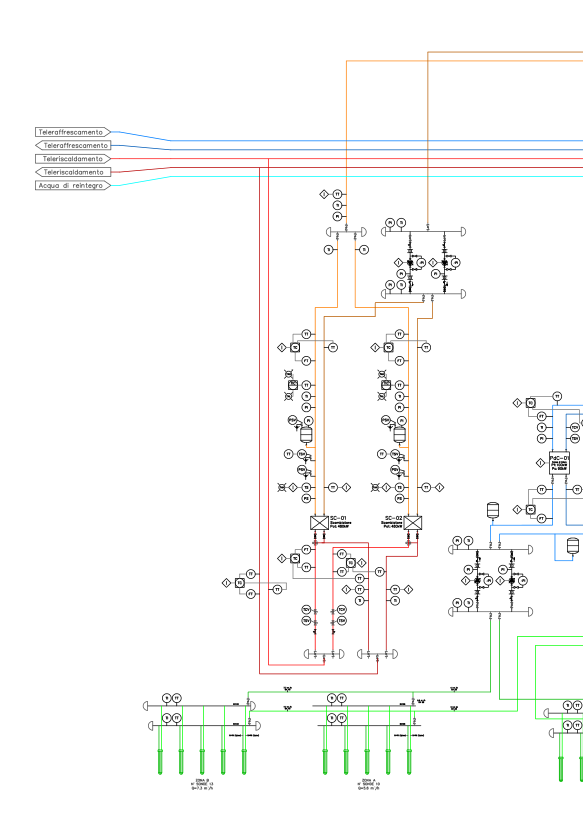
\includepdf{6_4_cap/img/sottocentr}
\begin{figure}
	\centering
	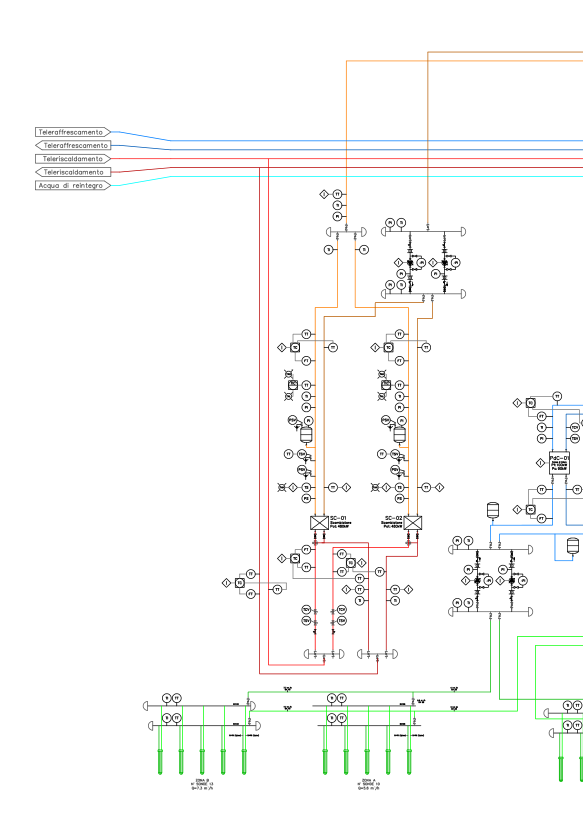
\includegraphics[width=\textwidth]{6_4_cap/img/sottocentr}
	\caption{Schema Sottocentrale -- Edificio 2}
	\label{img:sott}
\end{figure}
